\documentclass[a4paper,twoside]{article}
\usepackage{afterpage}
\usepackage{array} 
\usepackage{amsmath}
\usepackage{amssymb}
\usepackage{amsthm}
\usepackage{amstext} 
\usepackage{amsfonts}
\usepackage[english]{babel}
\usepackage{booktabs}
\usepackage{bm}
\usepackage{bbm}
\usepackage{caption}
\usepackage{contour}
\usepackage{csquotes}
\usepackage[shortlabels]{enumitem}
\usepackage{fancyhdr}
\usepackage{float}
\usepackage{fontenc}
\usepackage{fontspec}
\usepackage{geometry}
\usepackage{graphicx}
\usepackage{hhline}
\usepackage[hidelinks,unicode]{hyperref}
\usepackage[noabbrev]{cleveref}
\usepackage{longtable}
\usepackage{lmodern}
\usepackage{listings}
\usepackage{nicematrix}
\usepackage{mathtools}
\usepackage{multirow,array}
\usepackage{parskip}
\usepackage{pgfplots}
\pgfplotsset{compat=1.18}
\usepgfplotslibrary{dateplot}
\usepackage{ragged2e}
\usepackage[lm]{sfmath}
\usepackage{subcaption}
\usepackage{tabularx}
\usepackage{thmtools}
\usepackage{titlesec}
\usepackage{tikz}
\usetikzlibrary{intersections, angles, quotes, calc, positioning}
\usetikzlibrary{arrows.meta}
\usetikzlibrary{bending}
\tikzset{>=stealth}
\usepackage[theorems, skins, breakable]{tcolorbox}
\usepackage{wrapfig}
\usepackage{ulem}
\usepackage{xcolor}

%afterpage
\newcommand\blankpage{
	\null
	\pagestyle{fancy}
	\fancyhead{}\fancyfoot{}
	\fancyhead[RO,LE]{\thepage}
	\newpage}

%sff for all types of font
\renewcommand{\familydefault}{\sfdefault}

%uline setup
\setcounter{MaxMatrixCols}{20}
\renewcommand{\ULdepth}{2pt}
\contourlength{0.7pt}
\newcommand{\myuline}[1]{%
	\uline{\phantom{#1}}%
	\llap{\contour{white}{#1}}%
}

%image path
\graphicspath{ {./images/} }

%boxes
\newtcolorbox{questionbox}[1]{enhanced, breakable, colback=white, colbacktitle=myblue, colframe=myblue, title=#1,sharpish corners, fonttitle=\bfseries, boxrule=0pt, attach boxed title to top left={yshift=-2mm}}
\newtcolorbox{explanationbox}{enhanced, breakable, borderline west={2pt}{0pt}{myblue}, colback=myblue!5, boxrule=0pt,frame hidden}
\newtcolorbox{mybox}{goldstylecolor}

%custom color
\defaultfontfeatures {Ligatures = TeX}
\definecolor{myblue}{HTML}{224099}
\definecolor{mygreen}{HTML}{409922}
\definecolor{mygold}{HTML}{997b22}
\definecolor{myred}{HTML}{992240}
\definecolor{mypurple}{HTML}{7b2299}

%page setup
\geometry{
	left=2.54cm,
	right=2.54cm,
	top=2.54cm,
	bottom=2.54cm,
}

%headers and Footers
\pagestyle{fancy}
\fancyhead{}\fancyfoot{}
\fancyhead[RO,LE]{\thepage}
\fancyhead[RE]{\rightmark}
\fancyhead[LO]{\leftmark}

%math commands
\DeclareMathOperator{\sgn}{sgn}
\DeclareMathOperator{\id}{id}
\DeclareMathOperator{\im}{im}
\DeclareMathOperator{\pj}{Proj}
\DeclareMathOperator{\var}{Var}
\DeclareMathOperator{\cov}{Cov}

%theorems
\tcbset{
	bluestylecolor/.style={enhanced, sharp corners, breakable,colback=myblue!15, coltitle=myblue, frame hidden, boxrule=0pt, detach title, before upper=\tcbtitle\par\smallskip, fonttitle=\bfseries, borderline west={2pt}{0pt}{myblue}},
	bluestyleline/.style={enhanced, sharp corners, breakable, colback=white, coltitle=myblue, frame hidden, boxrule=0pt, detach title, before upper=\tcbtitle\par\smallskip,  fonttitle=\bfseries, borderline west={2pt}{0pt}{myblue}},
	redstylecolor/.style={enhanced, sharp corners, breakable, colback=myred!15, coltitle=myred, frame hidden, boxrule=0pt, detach title, before upper=\tcbtitle\par\smallskip, fonttitle=\bfseries, borderline west={2pt}{0pt}{myred}},
	redstyleline/.style={enhanced, sharp corners, breakable,colback=white, coltitle=myred, frame hidden, boxrule=0pt, detach title, before upper=\tcbtitle\par\smallskip, fonttitle=\bfseries, borderline west={2pt}{0pt}{myred}},
	greenstylecolor/.style={enhanced, sharp corners, breakable, colback=mygreen!15, coltitle=mygreen, frame hidden, boxrule=0pt, detach title, before upper=\tcbtitle\par\smallskip, fonttitle=\bfseries, borderline west={2pt}{0pt}{mygreen}},
	greenstyleline/.style={enhanced, sharp corners, breakable, colback=white, coltitle=mygreen, frame hidden, boxrule=0pt, detach title, before upper=\tcbtitle\par\smallskip, fonttitle=\bfseries, borderline west={2pt}{0pt}{mygreen}},
	goldstylecolor/.style={enhanced, sharp corners, breakable, colback=mygold!15, coltitle=mygold, frame hidden, boxrule=0pt, detach title, before upper=\tcbtitle\par\smallskip, fonttitle=\bfseries, borderline west={2pt}{0pt}{mygold}},
	goldstyleline/.style={enhanced, sharp corners, colback=white, colframe=mygold, boxrule=0pt,breakable, mygold=\bfseries, borderline horizontal={2pt}{0pt}{mygreen}},
}

\newtcbtheorem[number within=section, crefname={definition}{definitions}]{definition}{Definition}{greenstylecolor}{def}
\newtcbtheorem[use counter from=definition, crefname={theorem}{theorems}]{theorem}{Theorem}{goldstyleline}{tho}
\newtcbtheorem[use counter from=definition, crefname={lemma}{lemmas}]{lemma}{Lemma}{redstylecolor}{lem}
\newtcbtheorem[use counter from=definition, crefname={remark}{remarks}]{remark}{Remark}{bluestyleline}{rem}
\newtcbtheorem[use counter from=definition, crefname={corollary}{corollarys}]{corollary}{Corollary}{greenstyleline}{col}
\newtcbtheorem[use counter from=definition, crefname={example}{examples}]{example}{Example}{bluestylecolor}{exa}
\newtcbtheorem[use counter from=definition, crefname={proposition}{propositions}]{proposition}{Proposition}{redstyleline}{pro}
\newtcbtheorem[use counter from=definition, crefname={axiom}{Axiom}]{axiom}{Axiom}{goldstylecolor}{axm}

\tcbset{highlight math style={enhanced,colframe=mygold,colback=mygold!15,boxsep=0pt}}

\numberwithin{equation}{section}
\numberwithin{figure}{section}
\newcommand{\sectionbreak}{\clearpage}

%subsubsection
\titleformat{\subsubsection}{\bfseries}{}{0pt}{\myuline}
\titlespacing{\subsubsection}{0pt}{*3}{*1}

%preamble
\setcounter{tocdepth}{2}
\pagenumbering{roman}

\begin{document}
\begin{titlepage}
	\centering
	\vspace*{4.5cm}
	\rule{\linewidth}{2pt}
	\LARGE\textbf{ECOS3018}\\
	\vspace{0.5cm}
	\Huge\textbf{Economics of Growth}\\
	\rule{\linewidth}{2pt}
	\LARGE\textbf{Notes}\\
	\vspace{1.5cm}
	\Large Brendan Chow
	\vfill
\end{titlepage}
\newpage
\
\newpage
\tableofcontents
\newpage
\
\newpage
\pagenumbering{arabic}
\section{Introduction to Growth Theory}\label{sec:1}
\subsection{Growth, Distribution and Duality - One-Sector Case}
	\begin{alignat}{1}
		\underbrace{Y_c a_{cc}(1+g)}_{\text{total investment in corn}} + c_w L_c &= Y_c \label{eq:1.1}\\
		a_{cc} (1+g) + c_w l &= 1 \label{eq:1.2}
	\end{alignat}
	where
	\begin{itemize}
		\item \( Y_c \) is the gross output of corn
		\item \( L_c \) is total labour required
		\item \( c_w \) is corn consumption per unit of labour
		\item \( a_{cc} \) is the unit input requirement of corn in the production of corn 
		\item \( g \) is the rate of output of corn.
	\end{itemize}
	The price system is
	\begin{equation}
		p_c a_{cc} (1+r) + w_m l = p_c \label{eq:1.3}
	\end{equation}
	so that with corn as numeraire
	\begin{equation}
		a_{cc} (1+r) + wl = 1 \label{eq:1.4}
	\end{equation}
	The rate of profit (net profit of the value of commodity capital invested in production) associated with producing each unit of output is
	\begin{align}
		r &= \frac{p_c - w_m l - p_c a_{cc}}{p_c a_{cc}} \notag\\
		r &= \frac{1-wl-a_{cc}}{a_{cc}} 				 \label{eq:1.5}
	\end{align}
	Respectively equations (\ref{eq:1.2}) and (\ref{eq:1.4})
	\begin{alignat}{1}
		c_w &= \frac{1-a_{cc}(1+g)}{l} \label{eq:1.6}\\
		w   &= \frac{1-a_{cc}(1+r)}{l} \label{eq:1.7}
	\end{alignat}
	Note the symmetrical role of technical conditions in price and quantity systems. This is the duality of the price-quantity system. The maximum profit rate and the maximum growth rate are given by				
	\begin{equation}
		G = R = \frac{1-a_{cc}}{a_{cc}} \label{eq:1.8}
	\end{equation}
	At maximum consumption per worker \( g = 0 \); at maximum real wage \( r = 0 \), so that
	\begin{equation}
		c_{\max} = w_{\max} = \frac{1-a_{cc}}{l} \label{eq:1.9}
	\end{equation}
	If the term \( (1-s_p)ra_{cc}Y_c \) is included on the left hand side of \cref{eq:1.1}
	\[
		Y_c a_{cc} (1+g) + c_w L + (1-s_p)ra_{cc}Y_c = Y_c
	\]
	then, with \( c_w = w \)
	\[
		g = \frac{1-a_{cc}-wl}{a_{cc}}-(1-s_p)r
	\]
	while, from \cref{eq:1.5}
	\[
		r = \frac{1-a_{cc}-wl}{a_{cc}}
	\]
	so that
	\begin{equation}
		g = r-(1-s_p)r \implies g = s_p r \label{eq:1.10}
	\end{equation}
	Can arrive at \cref{eq:1.10} alternatively: assuming as before that all wages are spent
	\begin{equation}
		S = s_p \cdot P \label{eq:1.11}
	\end{equation}
	where
	\begin{itemize}
		\item \( s_p \) is planned savings
		\item \( P \) is profit
	\end{itemize}
	With planned saving equal to planned investment
	\begin{equation}
		I = s_p \cdot P \quad\text{and}\quad \frac{I}{K} = \frac{s_p \cdot P}{K} \label{eq:1.12}
	\end{equation}
	Assuming that output and the capital stock grow at the same rate, \( g \), then can decompose \cref{eq:1.10}
	\begin{equation}
		g = s_p r = \frac{S}{P}\frac{P}{Y}\frac{Y}{K} = \frac{S}{Y}\frac{Y}{K} = s \frac{Y}{K} \label{eq:1.13}
	\end{equation}
	so that, with
	\begin{equation}
		v = \frac{K}{Y} \label{eq:1.14}
	\end{equation}
	then
	\begin{equation}
		g = \frac{s}{v}
	\end{equation}
\subsection{Duality of Price and Quantity Systems in the Two-Sector Case}
	Consider the two-commodity ``iron-corn model'', where the economy is growing (uniformly across sectors) at the rate \( g \) per period
	Gross outputs for the two sectors are
	\begin{align}
		\underbrace{(Y_c a_{cc} + Y_i a_{ci})(1+g)}_{\text{total investment demand for corn}} + C_c &= Y_c \notag\\
		\underbrace{(Y_c a_{ic} + Y_i a_{ii})(1+g)}_{\text{total investment demand for iron}} + C_i &= Y_i \label{eq:1.16}
	\end{align}
	Suppose the growth rate is such that consumption per capita remains constant \( \implies \frac{C_{ct}}{N_t} = c_c \) remains constant where \( C_{ct} \) and \( N_t \) are corn consumption and population at time \( t \). We can also assume:
	\begin{itemize}
		\item in each period output corresponds to demand;
		\item there is only consumption demand for corn; \( C_i = 0 \)
		\item the labour force \( (L) \)  seeking work is a constant percentage of population \( (N) \)
		\item growth is sufficient to provide for full-employment of labour
		\[
			\frac{L_t}{N_t} \;\text{is constant and}\; l_c Y_{ct} + l_i Y_{it} = L_t
		\]
		\item \( \implies \frac{l_c Y_{ct} + l_i Y_{it}}{N_t} \) is constant
	\end{itemize}
	Consumption per worker can be expressed as
	\begin{equation}
		c_w = \frac{C_{ct}}{N_t}\frac{N_t}{l_c Y_{ct} + l_i Y_{it}} = c_c \frac{N_t}{l_c Y_{ct} + l_i Y_{it}} \label{eq:1.17}
	\end{equation}
	Defining output per capita as
	\[
		\frac{Y_{ct}}{N_t} = y_c \quad \frac{Y_{it}}{N_t} = y_i
	\]
	one can write \cref{eq:1.17} and solve for \( c_c \)
	\begin{equation}
		c_c = c_w(l_c y_c + l_i y_i) \label{eq:1.18}
	\end{equation}
	In turn, the quantity system (\ref{eq:1.16}) can be expressed as 
	\begin{align}
		(y_c a_{cc} + y_i a_{ci})(1+g) + c_w (l_c y_c + l_i y_i) &= y_c \notag \\
		(y_c a_{ic} + y_i a_{ii})(1+g) &= y_i \label{eq:1.19}
	\end{align}
	For a given structure or composition of output i.e. \( \frac{y_c}{y_i} = \frac{Y_c}{Y_i}\) , (\ref{eq:1.19}) yield the following relation betqeen \( g \) and \( c_w \)
	\begin{equation}
		c_w = \frac{(a_{cc}a_{ii} - a_{ci}a_{ic})(1+g)^2 - (a_{cc}+ a_{ii})(1+g)+1}{(l_i a_{ic} - l_c a_{ii})(1+g)+l_c} \label{eq:1.20}
	\end{equation}
	Consider the price system for this economy
	\begin{align}
		(a_{cc} p_c + a_{ic} p_i)(1+r) + w_m l_c &= p_c \notag \\
		(a_{ci} p_c + a_{ii} p_i)(1+r) + w_m l_i &= p_i \label{eq:1.21}
	\end{align}
	Note the uniform rate of profit.\\
	With corn as the numeraire
	\begin{align}
		(a_{cc} p_c + a_{ic} p_i)(1+r) + w_c l_c &= 1 \notag \\
		(a_{ci} p_c + a_{ii} p_i)(1+r) + w_c l_i &= p_{ic} \label{eq:1.22}
	\end{align}
	i.e \( w_c = \frac{w_m}{p_c} \), \( p_{ic} = \frac{p_i}{p_c} \). The real wage in terms of corn is given by
	\begin{equation}
		w_c = \frac{(a_{cc}a_{ii} - a_{ci}a_{ic})(1+r)^2 - (a_{cc}+ a_{ii})(1+g)+1}{(l_i a_{ic} - l_c a_{ii})(1+g)+l_c} \label{eq:1.23}
	\end{equation}
	Comparing with \cref{eq:1.20}, this is the duality of price and quantity system, for every technique yielding a \textit{w-r} relation there is a corresponding \textit{\( c_w \)-g} relation.\\
	The outmost envelope of the set of \textit{\( c_w \)-g} represents the technological frontier of consumption-growth possibilities
	\begin{figure}[H]
		\centering
		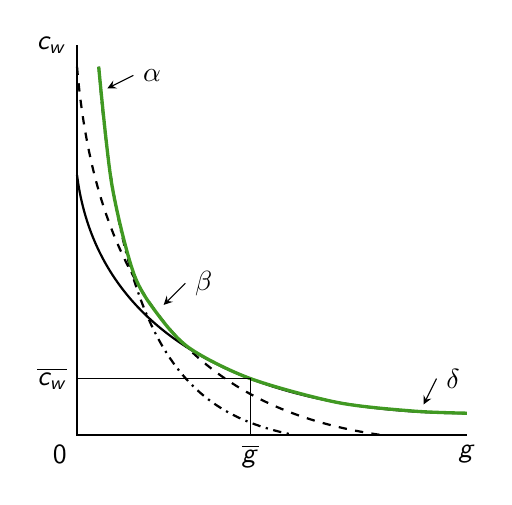
\begin{tikzpicture}[scale=0.55]
			\draw [thick] (0,9) node[left]{\(c_w\)} -- (0,0) node[below left]{0} -- (9,0) node[below]{\(g\)};
			\draw [thick] (0,6) .. controls (0.5,2) and (4.5,0.5) .. (9,0.5);
			\draw[<-] (8,0.7) -- (8.3,1.3) node[right]{\( \delta \)};
			\draw [thick,dashed] (0,8.5) .. controls (0.5,2.5) and (3.5,0.5) .. (7,0);
			\draw[<-] (2,3) -- (2.5,3.5) node[right]{\( \beta \)};
			\draw [thick,dash dot] (0.5,8.5) .. controls (1,2) and (2.5,0.5) .. (5,0);
			\draw[<-] (0.7,8) -- (1.3,8.3) node[right]{\( \alpha \)};
			\draw [smooth,very thick,color=mygreen] plot coordinates {(0.5,8.5)(0.8,5.8)(1.3,3.75)(1.85,2.8)(2.6,2)(4,1.3)(6,0.75)(7.75,0.55)(9,0.5)};
			\draw (0,1.3) node [left] {\(\overline{c_w}\)}-- (4,1.3) -- (4,0) node [below]{\( \overline{g} \)};
		\end{tikzpicture}
		\caption{Technological Frontier of Consumption-Growth Possibilities}
	\end{figure}
	At a given growth rate, e.g. \( \overline{g} \) the corresponding point on the frontier indicates the technique which maximises \( c_w \) for that growth rate.\\
	\begin{itemize}
		\item Preceding analysis assumes that \( g \) is determined by the requirement of full-employment.
		\item To the extent that one relaxes this assumption, this leaves up in the air the determination of \( g \).
		\item Traditional orthodox growth theory accepts the notion that long-run growth will be consistent with the requirements of full-employment.
		\item Analogous arguments to those used in a static context (i.e. for a stationary economy).
		\item However, the history of formal growth theory (mainly through the 20th century) contains a rich undercurrent of dissent from this view.
	\end{itemize}
\afterpage{\blankpage}

\section{Early Keynesian-Inspired Models of Growth: Harrod and Domar}
\subsection{A Conceptual Issue in Moving to Growth Analysis: the Two Sides of Investment}
	\begin{itemize}
		\item Simple Keynesian multiplier (ignore autonomous components of planned aggregate expenditure (AE) other than investment):  
	\begin{equation}
		\textcolor{mygold}{Y} = AE = \frac{1}{1-c}I \label{eq:2.1}
	\end{equation}
	\item Given \( c \), constant \( I \implies \) constant level of expenditure. Thus the equilibrium \( Y \) is constant - a ``stationary equilibrium'' (i.e \( Y = AE \)).
	\item But suppose \( I \) includes positive net invest \( \implies \) productive capacity is expanding. Producers must be anticipating growth in demand. How is this consistent with a constant \( AE \)?
	\item With demand constant producers would find their productive capacity underutilized. For equilibrium, increased output produced with larger capacity must be matched by increased demand. With positive net investment equilibrium requires that aggregate demand grow in line with productive capacity. From \cref{eq:2.1}, if \( c \) is constant, \( I \) must be growing, so according to \cref{eq:2.1}, \( Y \) must be growing - a ``moving equilibrium''.
	\item Hence, with a positive net investment, it is incorrect to speak of equilibrium \textbf{level} of income. The appropriate concept is instead an equilibrium \textbf{rate of growth} of income.
	\begin{mybox}
		Taking account of two sides of investment \( \implies \) equilibrium must be one characterised by growing output. Along the equilibrium growth path, the demand effects from growing investment exactly balance capacity effects from that investment
	\end{mybox}
	\item In other words, produces expand capacity by \( x\% \) via increases investment on the basis of an expected expansion of demand at \( x\% \).
	\item Increased investment orders \( \implies \) a multiplied increase in aggregate expenditure
	\begin{equation}
		\Delta AE = \frac{1}{1 - c} \Delta I \label{eq:2.2}
	\end{equation}
	\item \textbf{Along the equilibrium growth path}, AE will actually expand by the rate which producers expected -- i.e. \( x\% \) -- thereby justifying the \( x\% \) expansion in capacity 
	\item \( \implies \) demand effects of expanding investment exactly match the capacity effects.
	\end{itemize}
\subsection{The Harrod-Domar Approach}
	\begin{itemize}
		\item Can be seen as an attempt to extend Keynes's ``principle of effective demand'' (PED) (1936) into the ``long-run'', i.e. to a growing economy. 
		\item PED is the level of output and employment are ultimately constrained by the level of aggregate demand in a capitalist economy -- i.e. the effective limit on the level of output and employment is \textbf{\myuline{not}} the full-employment of labour, either in the short-run or the long-run.
		\item Alternatively put, investment governs the level of saving and there is no mechanism to ensure investment will be sufficient to warrant the full-employment level of output (i.e. to absorb the level of saving at the full-employment level of income).
		\item The simple multiplier can be used to illustrate
		\begin{align}
			\Delta Y = \frac{1}{1-c} \Delta I \implies \Delta S &= (1-c) \Delta Y\\ \notag
																&= \frac{1-c}{1-c} \Delta I\\ \notag
																&= \Delta I \label{eq:2.3}
		\end{align}
		\item An autonomous increase in \( I \) generates sufficient change in \( Y \), such that, given the propensity to save out of income \( l-c \), \( S \) increases by a matching amount. 
		\item Keynes's own formal statement dealt with a stationary economy -- i.e. a given capital stock -- thereby ignoring capacity effects of investment. 
		\item But taking account of these effects \( \implies \) need to recast the analysis for a growing economy.
		\item In essence both Harrod and Domar start with the following question: 
		\begin{quote}
			is there a rate of growth of output which would be self-sustaining in the sense that producers would be content to continue expanding capacity at that rate?
		\end{quote}
		\item Such a rate would require capacity and demand effects of growing investment to balance. From the multiplier relation
		\begin{equation}
			Y = \frac{1}{s} I \implies \Delta Y = \frac{1}{s} \Delta I \implies \Delta I = s \Delta Y \label{eq:2.4}
		\end{equation}
		\item Taking \( v \) as the desired ``marginal'' capital to output ratio, the accelerator is
		\begin{equation}
			I = v \Delta Y \implies \Delta K = v \Delta Y \label{eq:2.5}
		\end{equation}
		\item Combining \cref{eq:2.4} and \ref{eq:2.5}:\\
		Firstly
		\[
			\Delta I = s \Delta Y \quad\text{and}\quad I = v \Delta Y
		\]
		Secondly
		\[
			Y = \frac{1}{s} I \quad\text{and}\quad I = v \Delta Y
		\]
		Therefore
		\begin{equation}
			\frac{\Delta I}{I} = \frac{s}{v} = \frac{\Delta Y}{Y} = g_w \label{eq:2.6}
		\end{equation}
		\item \( g_w \) is the equilibrium or ``warranted'' (Harrod) growth rate.
		\item Assume investment orders grow at this rate and producers utilize their expanding capacity so as to maintain the desired ratio of output to the capital stock equal to `\( \frac{1}{v} \)'. 
		\item ``On balance'', according to Harrod, the growing demand generated through the multiplier process by growing investment orders will match the growing output produced with the expanding capital stock.
		\item The growth in investment orders  and the consequent expansion of the capital stock will have been ``warranted'' (i.e. justified) by the growth in AE generated by those same investment orders. 
		\item In effect, producers' expectations about future demand growth - on which investment is based -- will have been realised.
		\item Along the warranted growth saving will adapt to growing investment via changes in output brought about by expanding productive capacity.
		\item Since \( S = sY, \Delta S = s \Delta Y \) then
		\begin{equation}
			\frac{\Delta S}{S} = \frac{\Delta Y}{Y} = \frac{\Delta I}{I} \label{eq:2.7}
		\end{equation}
		\item Contrast with ``static'' Keynesian multiplier case where \( Y \) changes to bring \( S \) into line with \( I \) with given \( K \).
		\item Along with the warranted path \( K \) is also growing.
		\item For Harrod, stable equilibrium growth consistent with continuous full-employment requires equality of actual, natural and warranted growth rates:
		\begin{equation}
			g_a = g_n = g_w \label{eq:2.8}
		\end{equation}
		where
		\begin{itemize}
			\item \( g_a \) is the actual growth rate
			\item \( g_n \) natural growth rate
			\item \( g_w \) warranted growth rate
		\end{itemize}
		\item \( g_n = g_a \) required for the maintenance of full-employment
		\item \( g_n \) set maximum for \( g_a \)\\
		\item According to Harrod, the warranted growth path is an unstable equilibrium
		\item i.e. where \( g_a \neq g_w \) the gap between \( g_a \) and \( g_w \) increases.
		\item Along the warranted growth path
		\begin{equation}
			g_a = \left( \frac{I}{K} \right)_{\text{actual}} = g_w = \frac{s}{v} = \frac{S}{Y} \frac{Y}{K} = \frac{S}{K} \label{eq:2.9}
		\end{equation}
		\item e.g. consider the case \( g_a > g_w \) 
		\begin{align*}
			&\left( \frac{I}{K} \right)_{\text{actual}} > \frac{s}{v} \quad \left( \frac{I}{K} \right)_{\text{actual}} > \frac{S}{K} \\ 
			\implies &\left( \frac{Y}{K} \right)_{\text{actual}} > \left( \frac{Y}{K} \right)_{\text{warranted}}
		\end{align*}
		It implies that actual demand growth exceeds expected demand growth.
		Effectively two cases:
		\begin{enumerate}[(a)]
			\item \( g_w > g_n \). Since \( g_a \leq g_n \) then \( g_a < g_w \).\\
				Hence, given the saving ratio and desired capital to output ratio, the growth of investment required for equilibrium is greater than the maximum possible \( \implies \) chronic tendency to unemployment.
			\item \( g_w < g_n \). Two possibilities arise:
			\begin{itemize}[(i)]
				\item \( g_w < g_a \leq g_n \implies \) capacity continually overutilized \( \implies \) growth rate of investment continually pressing against the full-employment ceiling \( \implies \) inflationary pressures.
				\item \( g_a \leq g_w < g_n \). Either mounting unemployment in the special case where \( g_a = g_w \) and thus \( g_a < g_n \).\\
				or, \( g_a < g_w \) and hence case (a) above and therefore chronic unemployment.
			\end{itemize}
		\end{enumerate}
	\end{itemize}
\afterpage{\blankpage}

\section{Traditional Neo-Classical Growth Theory: Solow-Swan}
\subsection{Growth Without Technical Progress}
	\begin{itemize}
		\item Assume constant returns to scale production technology using capital and labour:
		\begin{equation}
			Y = F(K,L) = AK^\alpha L^\beta \label{eq:3.1}
		\end{equation}
		\item Assume \( \alpha + \beta = 1 \implies \alpha = 1 - \beta \). In per worker terms (dividing through by \( L \))
		\begin{equation}
			\frac{Y}{L} = \frac{AK^\alpha L^\beta}{L} = AK^{1-\beta} L^{-(1-\beta)} = \frac{AK^{1-\beta}}{L^{1-\beta}} = \frac{AK^\alpha}{L^\alpha} \label{eq:3.2}
		\end{equation}
		\begin{equation}
			\therefore y = Ak^\alpha \quad\text{where}\; k=\frac{K}{L},\;\text{or}\quad y=f(k) \label{eq:3.3}
		\end{equation}
		\item Ignore technical progress \( \implies \) in equilibrium output and the capital stock grow at the same rate, \( g_e \)
		\item Ignoring physical depreciation, \( \%\Delta K \frac{I}{K} \) with depreciation at the rate \( \delta \implies \% \Delta K = \frac{I}{K} -\delta \)
		\item In this model, \( g_e = g_n \) (i.e. \( \%\Delta \) working age population)
		\item i.e. in equilibrium, output and the capital stock grow at the same rate as the labour force
		\begin{equation}
			g_e = \frac{\Delta Y}{Y} = \frac{I}{K} = \frac{s}{v} = \frac{S}{Y} \frac{Y}{K} = g_n \label{eq:3.4}
		\end{equation}
		\item Writing for \( v \),
		\begin{equation}
			v = \frac{K}{Y} = \frac{K}{L}\frac{L}{Y} = \frac{k}{y} \therefore s \frac{y}{k} = g_n \label{eq:3.5}
		\end{equation}
		\begin{equation}
			\implies s \frac{f(k)}{k} = g_n \label{eq:3.6}
		\end{equation}
		\begin{equation}
			\tcbhighmath{sf(k) = sy = g_n k} \quad\text{or}\quad \tcbhighmath{f(k) = \frac{g_n k}{s}} \label{eq:3.7}
		\end{equation}
		\item An example: assume \( g_L = g_n \)  (i.e. labour employment grows at the same rate as the labour force -- why this is, we will take up shortly). 
		\item Suppose at a point time \( K = 1000, L = 100 \), therefore \( k=10, \) and \( g_L = 0.2 = g_n \).
		\item To keep \( k \) constant requires, \( g_n k \) investment per worker. 
		\item \( 0.2(\frac{1000}{100} = 2) \) units of capital of investment per worker.
		\item \Cref{eq:3.6} and (\ref{eq:3.7}) imply that \( s \frac{Y}{L} = sy \) (i.e saving per worker) must be equal to 2 in order to keep \( k \) constant i.e. if \( sy = g_n k \), \( k \) will be constant.
		\item With \( k \) constant, \( y \) is constant, given \( f(k) \).
		\item From \cref{eq:3.6}
		\begin{equation}
			s \frac{f(k)}{k} = g_n \implies s \frac{Y/L}{K/L} = g_n \implies \frac{sY}{K} = \frac{I}{K} = g_n
		\end{equation}
		\item Along the equilibrium path, \( S,I,Y \) and \( K \) all grow at the same rate - \( g_n \)
		\item Where \( \delta > 0 \frac{I}{K}-\delta = g_n \) in the steady state; and hence
		\[
			s \frac{Y}{K} - \delta = g_n \quad\text{and}\quad s \frac{y}{k} = g_n + \delta
		\]
		so that \cref{eq:3.7} becomes \( sy = (g_n + \delta)k \) 
		\begin{figure}[H]
			\centering
			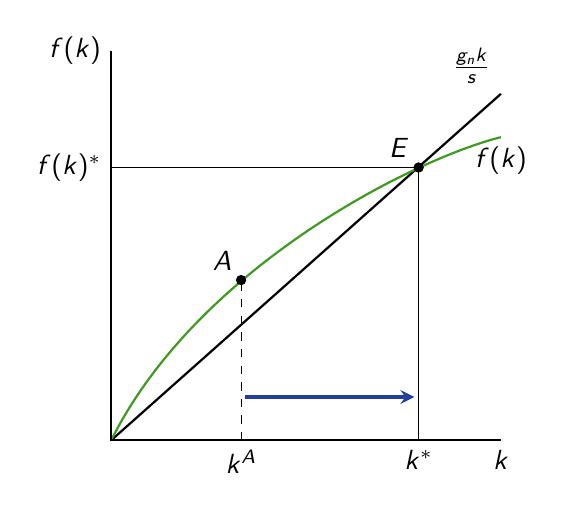
\begin{tikzpicture}[scale=0.55]
				\draw [thick] (0,0) -- (9,8) node[above left]{\( \frac{g_n k}{s} \)};
				\draw [thick, mygreen] (0,0) .. controls (2,4) and (7,6.5) .. (9,7) node[below,black]{\( f(k) \)};
				\draw (0,6.3) node[left]{\( f(k)^\ast \)} -- (7.1,6.3) node[above left]{\( E \)} -- (7.1,0) node[below]{\( k^\ast \) };
				\filldraw[black] (7.1,6.3) circle (3pt);
				\draw [dashed] (3,0) node[below]{\( k^A \) } -- (3,3.7) node[above left]{\( A \)};
				\filldraw[black] (3,3.7) circle (3pt);
				\draw [very thick, myblue, ->] (3.1,1) -- (7,1);
				\draw [thick] (0,9) node[left]{\(f(k)\)} -- (0,0) -- (9,0) node[below]{\(k\)};
			\end{tikzpicture}
		\end{figure}
		\item At \( k^A \),
		\begin{equation}
			f(k) > \frac{g_n k}{s} \implies s \frac{f(k)}{k} > g_n \implies \frac{I}{K} > g_n \tag{3.9a}\label{eq:3.9a}
		\end{equation}
		\item Note \( g_L < g_n \)
		\item If \( \frac{\Delta K}{K} > g_n \), then \( \frac{\Delta K}{K} > g_L \implies \uparrow k \)
		\item At \( E, f(k) = \frac{g_n k}{s} \) 
		\item \( \implies \) if \( g_n \) is exogenous, the transition from \( A \) to \( E \) (and thus the rise) in \( k \) from \( k^A \to k^\ast \) must result in a fall in \( \frac{I}{K} \).
		\begin{figure}[H]
			\centering
			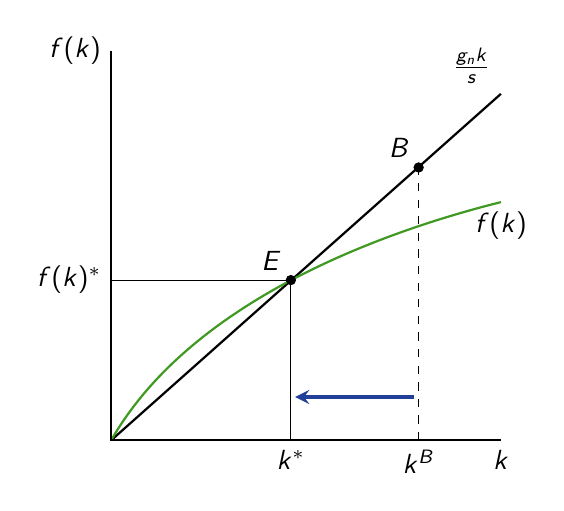
\begin{tikzpicture}[scale=0.55]
				\draw [thick] (0,0) -- (9,8) node[above left]{\( \frac{g_n k}{s} \)};
				\draw [thick, mygreen] (0,0) .. controls (2,3.5) and (7,5) .. (9,5.5) node[below,black]{\( f(k) \)};
				\draw (0,3.7) node[left]{\( f(k)^\ast \)} -- (4.15,3.7)  node[above left]{\( E \)} -- (4.15,0) node[below]{\( k^\ast \) };			
				\filldraw[black] (4.15,3.7) circle (3pt);
				\draw [dashed] (7.1,0) node[below]{\( k^B \)} -- (7.1,6.3) node[above left]{\( B \)};
				\filldraw[black] (7.1,6.3) circle (3pt);
				\draw [very thick, myblue, <-] (4.25,1) -- (7,1);
				\draw [thick] (0,9) node[left]{\(f(k)\)} -- (0,0) -- (9,0) node[below]{\(k\)};
			\end{tikzpicture}
		\end{figure}
		\item At \( k^B \),
		\begin{equation}
			f(k) < \frac{g_n k}{s} \implies s \frac{f(k)}{k} < g_n \implies \frac{I}{K} < g_n \tag{3.9b}\label{eq:3.9b}
		\end{equation}
		\item If \( g_L < g_n \implies \) rising unemployment, \( \downarrow w \) and incentive to reduce \( k \).
		\item If \( g_L = g_n \), while \( \frac{\Delta K}{K} < g_{n, k} \) would be falling.
		\item Transition from \( B \) to \( E \)  (and thus fall in \( k \) from \( k^B \to k^\ast \)) results in a rise in \( \frac{I}{K} \) so that at \( E \)
		\[
			f(k) = \frac{g_n k}{s}
		\]
		\item At the steady state k = k*, there must be no incentive to alter k, i.e. to alter the employment of capital relative to labour. 
		\item This implies no pressure on real wages via excess demand or supply in the labour market. In turn, this requires full-employment and growth of labour employment equal to the rate of growth of the labour force. 
		\item i.e. \( g_L = g_n \)
	\end{itemize}
\subsection{Diminishing Returns and the Steady State}
	\begin{itemize}
		\item Falling marginal and average productivities \( \implies \downarrow \frac{\Delta Y}{\Delta K} \) and \( \downarrow \frac{Y}{K} \) as \( \uparrow k \)
		\begin{figure}[H]
			\centering
			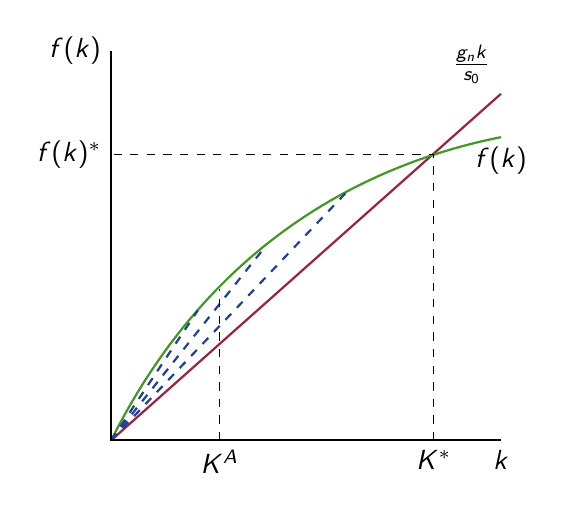
\begin{tikzpicture}[scale=0.55]
				\draw [thick, myred] (0,0) -- (9,8) node[above left, black]{\( \frac{g_n k}{s_0} \)};
				\draw [thick, mygreen] (0,0) .. controls (2.5,5) and (6.5,6.5) .. (9,7) node[below, black]{\( f(k) \)};
				\draw [thick, dashed, myblue] (0,0) -- (2,3);
				\draw [thick, dashed, myblue] (0,0) -- (3.5,4.4);
				\draw [thick, dashed, myblue] (0,0) -- (5.5,5.8);
				\draw [thick] (0,9) node[left]{\(f(k)\)} -- (0,0) -- (9,0) node[below]{\(k\)};
				\draw [dashed] (2.5,0) node[below]{\( K^A \)} -- (2.5,3.5);
				\draw [dashed] (7.45,0) node[below]{\( K^\ast \)} -- (7.45,6.6) -- (0,6.6) node[left]{\( f(k)^\ast \)};
			\end{tikzpicture}
		\end{figure}
		\item e.g. at \( k^A \), \( \uparrow k \implies \downarrow \frac{Y}{K} \implies \frac{sY}{K} \downarrow \implies \downarrow \frac{I}{K} \implies \downarrow \frac{\Delta K}{K} \) until \( k \) stops rising at \( k^\ast \) where \( \frac{\Delta K}{K} = g_n \)
	\end{itemize}
\subsection{Growth and Income Distribution}
	\begin{itemize}
		\item The constant returns to scale production function (\ref{eq:3.1}) can be rewritten as
		\begin{equation}
			Y = \frac{\partial Y}{\partial L} L + \frac{\partial Y}{\partial K} K \tag{3.10}\label{eq:3.10}
		\end{equation}
		\item Assuming factors are paid their marginal products
		\item \( \implies Y = wL + rK \)
		\begin{equation}
			y = w + rk \tag{3.11}\label{eq:3.11}
		\end{equation}
		\item \( \implies \) income consists of wages and profit
		\begin{figure}[H]
			\centering
			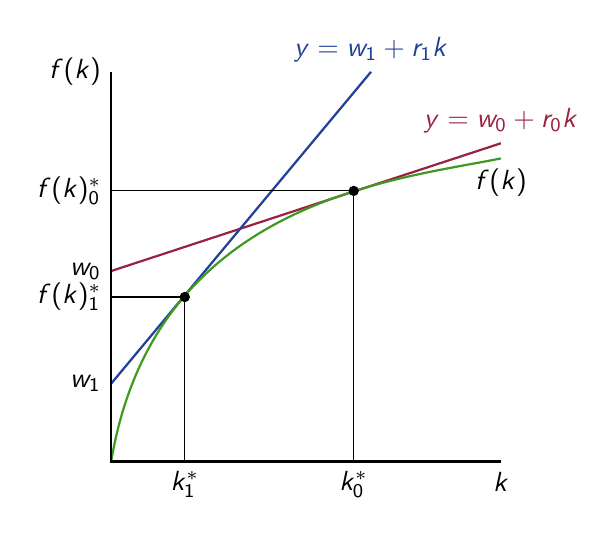
\begin{tikzpicture}[scale=0.55]
				\draw [thick, myred] (0,4.4) node[left, black]{\( w_0 \)} -- (9,7.35) node[above]{\( y = w_0 + r_0 k \)};
				\draw [thick, myblue] (0,1.8) node[left, black]{\( w_1 \)} -- (6,9) node[above]{\( y = w_1 + r_1 k \)};
				\draw [thick, mygreen] (0,0) .. controls (1,6) and (6.5,6.5) .. (9,7) node[below, black]{\( f(k) \)};
				\draw [black] (0,3.8) node[left]{\(f(k)_1^{\ast} \)} -- (1.7,3.8) -- (1.7,0) node[below]{\( k_1^{\ast} \)};
				\filldraw[black] (1.7,3.8) circle (3pt);
				\draw [black] (0,6.25) node[left]{\(f(k)_0^{\ast} \)} -- (5.6,6.25) -- (5.6,0) node[below]{\( k_0^{\ast} \)};
				\filldraw[black] (5.6,6.25) circle (3pt);
				\draw [thick] (0,9) node[left]{\(f(k)\)} -- (0,0) -- (9,0) node[below]{\(k\)};
			\end{tikzpicture}
		\end{figure}
		\item Note the implications of marginal productivity theory regarding the connection between production, distribution and growth.
		\item A higher \( k \) (lower \( \frac{L}{K} \)) is associated with a lower profit rate and a higher real wage.
		\item Consider an \( \uparrow \) in \( g_n \implies \frac{g_n k}{s} \) line pivots to the left.
		\item New steady state at \( B \): higher growth rate; lower \( y,k \) and \( v \) lower \( w \), higher \( r \)
		\item Note: equilibrium growth rate in the Solow-Swan model is given by \( g_e = \frac{s}{v} = g_n \).
		\begin{figure}[H]
			\centering
			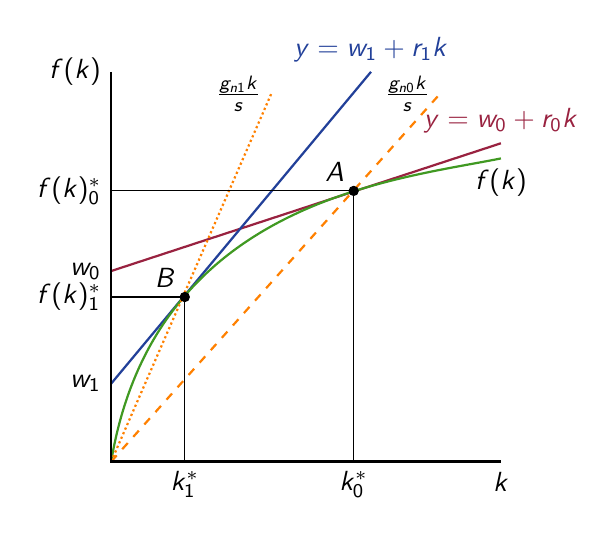
\begin{tikzpicture}[scale=0.55]
				\draw [thick, myred] (0,4.4) node[left, black]{\( w_0 \)} -- (9,7.35) node[above]{\( y = w_0 + r_0 k \)};
				\draw [thick, myblue] (0,1.8) node[left, black]{\( w_1 \)} -- (6,9) node[above]{\( y = w_1 + r_1 k \)};
				\draw [thick, mygreen] (0,0) .. controls (1,6) and (6.5,6.5) .. (9,7) node[below, black]{\( f(k) \)};
				\draw [thick, orange, densely dotted] (0,0) -- (3.7,8.5) node[left, black]{\( \frac{g_{n1}  k}{s} \)};
				\draw [thick, orange, dashed] (0,0) -- (7.6,8.5) node[left, black]{\( \frac{g_{n0}  k}{s} \)};
				\draw [black] (0,3.8) node[left]{\(f(k)_1^{\ast} \)} -- (1.7,3.8) -- (1.7,0) node[below]{\( k_1^{\ast} \)};
				\filldraw[black] (1.7,3.8) circle (3pt) node[above left]{\( B \)};
				\draw [black] (0,6.25) node[left]{\(f(k)_0^{\ast} \)} -- (5.6,6.25) -- (5.6,0) node[below]{\( k_0^{\ast} \)};
				\filldraw[black] (5.6,6.25) circle (3pt) node[above left]{\( A \)};
				\draw [thick] (0,9) node[left]{\(f(k)\)} -- (0,0) -- (9,0) node[below]{\(k\)};
			\end{tikzpicture}
		\end{figure}
		\item In this case, an \( \uparrow g_n \implies \uparrow g_e \). 
		\item But for this to be consistent with the fact that the equilibrium growth rate is equal to \( \frac{s}{v} \), either `\( s \)' or `\( v \)' must change.
		\item For a given `\( s \)', `\( v \)' must fall.
		\item Contrast this with Harrod: both `\( s \)' and `\( v \)' are fixed \( \implies \) if \( g_n \) rises above \( \frac{s}{v} \) there is no automatic mechanism to push \( \frac{s}{v} \) in line with the higher \( g_n \)
		\item Consider a rise in the savings ratio, \( s_0 \to s_1 \)
		\begin{figure}[H]
			\centering
			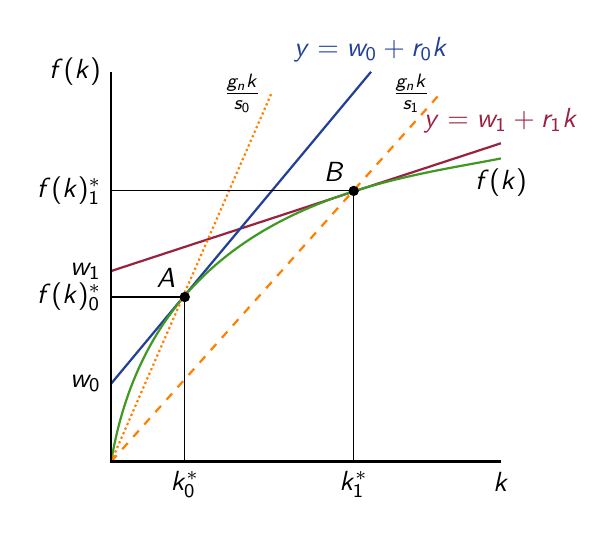
\begin{tikzpicture}[scale=0.55]
				\draw [thick, myred] (0,4.4) node[left, black]{\( w_1 \)} -- (9,7.35) node[above]{\( y = w_1 + r_1 k \)};
				\draw [thick, myblue] (0,1.8) node[left, black]{\( w_0 \)} -- (6,9) node[above]{\( y = w_0 + r_0 k \)};
				\draw [thick, mygreen] (0,0) .. controls (1,6) and (6.5,6.5) .. (9,7) node[below, black]{\( f(k) \)};
				\draw [thick, orange, densely dotted] (0,0) -- (3.7,8.5) node[left, black]{\( \frac{g_n k}{s_0} \)};
				\draw [thick, orange, dashed] (0,0) -- (7.6,8.5) node[left, black]{\( \frac{g_n k}{s_1} \)};
				\draw [black] (0,3.8) node[left]{\(f(k)_0^{\ast} \)} -- (1.7,3.8) -- (1.7,0) node[below]{\( k_0^{\ast} \)};
				\filldraw[black] (1.7,3.8) circle (3pt) node[above left]{\( A \)};
				\draw [black] (0,6.25) node[left]{\(f(k)_1^{\ast} \)} -- (5.6,6.25) -- (5.6,0) node[below]{\( k_1^{\ast} \)};
				\filldraw[black] (5.6,6.25) circle (3pt) node[above left]{\( B \)};
				\draw [thick] (0,9) node[left]{\(f(k)\)} -- (0,0) -- (9,0) node[below]{\(k\)};
			\end{tikzpicture}
		\end{figure}
		\item New steady state associated with same growth rate, but higher \( y,k \) and \( v \) (lower \( \frac{Y}{K} \)). 
		\item Adjustment to new steady state involves involves a transition to a higher real wage (move to a lower \( \frac{L}{K} \)) and a lower rate of profit.
		\item Note again how this contrasts with Harrod's analysis. 
		\item In the Solow-Swan case, \( \frac{s}{v} = g_n \). \( \frac{s}{v} \) adapts to \( g_n \implies \) with a given \( g_n \), if '\( s \)' rises, '\( v \)' rises so that \( \frac{s}{v} \) remains equal to \( g_n \).
		\item For Harrod an increase is '\( s \)' with a given '\( v \)' increases the warranted rate \( g_w \). 
		\item If \( g_w \)  rises above \( g_n \) the economy would suffer from a chronic tendency to unemployment	
	\end{itemize}

\section{Optimality and Growth Theory}
\subsection{Growth, Saving and the ``Golden Rule''}
	\begin{itemize}
		\item What is the impact of different saving ratios on the level of consumption in a growing economy?
		\item Consider this in the context of the Solow-Swan model: how is the steady state consumption per head affected by changing the saving ratio?
		\item The '\( k^\ast \)' and '\( s \)' associated with the highest steady state consumption per head known as the \textit{golden-rule} case.
		\item Steady state consumption per worker can be expressed as
		\begin{equation}
			f(k^\ast) - sf(k^\ast) = c^\ast = f(k^\ast) - g_n k^\ast \label{eq:4.1}
		\end{equation}
		\item To find the maximum \( c^\ast \) set
		\begin{equation}
			\frac{\mathrm{d}c^\ast}{\mathrm{d}k^\ast} = 0 \implies \frac{\mathrm{d}c^\ast}{\mathrm{d}k^\ast} = f^\prime(k^\ast) - g_n = 0 \label{eq:4.2}
		\end{equation}
		and thus
		\begin{equation}
			MP_k = g_n \label{eq:4.3}
		\end{equation}
		which is \textcolor{myblue}{\textbf{``golden rule''}}
		\item Thus consumption per worker and hence (with a fixed ratio of \( L \) to \( N \)) consumption per capita is maximised where the marginal product of capital is equal to the growth rate (\( g_n \) in the Solow-Swan model)
		\item In the Solow-Swan model
		\begin{equation}
			k^\ast = \frac{sf(k^\ast)}{g_n} \label{eq:4.4}
		\end{equation}
		\item \( \implies \) if \( g_n \) is fixed and the production function is unchanging, \( k^\ast \) is determined by `\( s \)'
		\item \( \implies \) `\( s \)' has to ``adjust'' to generate a \( k^\ast \) consistent with \( MP_K = g_n \) 
		\item This golden rule also implies a connection between distribution and growth
		\item Assuming \( MP_K = r \), this rule implies \( r = g_n \)
		\item Different values of `\( s \)' imply different \( k^\ast \)'s and \( MP_K \)'s and hence different \( r \)'s, for a given technology and given \( g_n \)
		\item One of these `\( s \)' will imply \( r = g_n \) 
	\end{itemize}
	\begin{figure}[H]
		\centering
		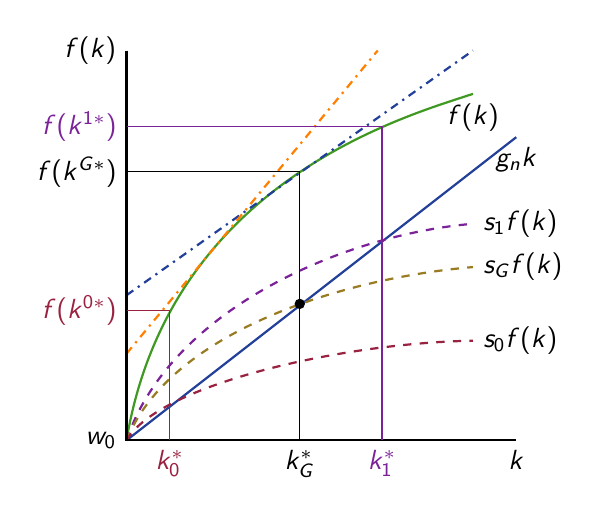
\begin{tikzpicture}[scale=0.55]
			\draw [thick, myblue] (0,0) node[left, black]{\( w_0 \)} -- (9,7) node[below, black]{\( g_n k \)};
			\draw [thick, mygreen] (0,0) .. controls (1,6) and (6.5,7.5) .. (8,8) node[below, black]{\( f(k) \)};
			\draw [thick, mypurple, dashed] (0,0) .. controls (1,3) and (5,4.75) .. (8,5) node[right, black]{\( s_1f(k) \)};
			\draw [thick, mygold, dashed] (0,0) .. controls (1,2.5) and (5,3.75) .. (8,4) node[right, black]{\( s_Gf(k) \)};
			\draw [thick, myred, dashed] (0,0) .. controls (0.75,1.3) and (5,2.25) .. (8,2.3) node[right, black]{\( s_0f(k) \)};
			\draw [thick, dash dot, myblue] (0,3.35) -- (8,9);
			\draw [thick, dash dot, orange] (0,2) -- (5.8,9);
			\draw [thick] (0,9) node[left]{\(f(k)\)} -- (0,0) -- (9,0) node[below]{\(k\)};
			\draw [myred] (1,0) node[below]{\( k_0^{\ast} \)} -- (1,3) -- (0,3) node[left]{\( f(k^{0\ast}) \)};
			\draw [mypurple] (5.9,0) node[below]{\( k_1^{\ast} \)} -- (5.9,7.25) -- (0,7.25) node[left]{\( f(k^{1\ast}) \)};
			\draw (4,0) node[below]{\( k_G^{\ast} \)} -- (4,6.2)  -- (0,6.2) node[left]{\( f(k^{G\ast}) \)};
			\filldraw[black] (4,3.15) circle (3pt);
		\end{tikzpicture}
	\end{figure}
	\begin{itemize}
		\item With \( s_0 \implies k^{0^\ast} \) and \( MP_K > g_n \) 
		\item \( \implies \) for a small \( \uparrow \) in \( k \), the \( \uparrow \) in \( y \) exceeds the \( \uparrow \) in saving and investment per worker required for the new higher \( k \implies \) allows for an \( \uparrow c^\ast \)
		\item But higher \( k^\ast \) requires, ceterius paribus, a higher \( s \)
		\item With \( s_1 = k^{l^\ast} \) and \( MP_K < g_n \)
		\item \( \implies \) small \( \downarrow \) in \( k \implies \downarrow \) in \( y < \downarrow \) in required saving and investment per worker \( \implies \uparrow c^\ast \) 
	\end{itemize}
	\begin{figure}[H]
		\centering
		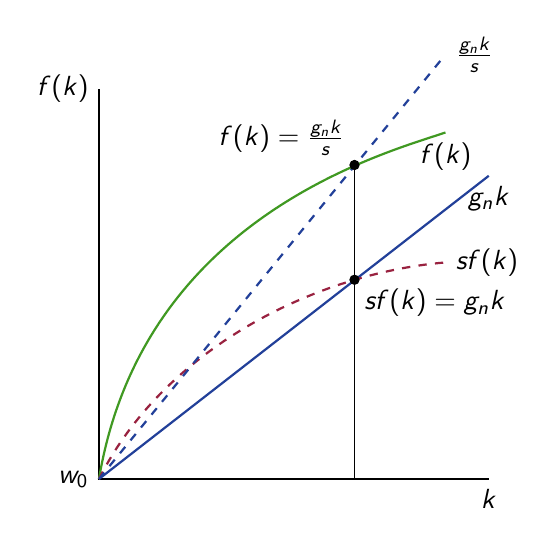
\begin{tikzpicture}[scale=0.55]
			\draw [thick] (0,9) node[left]{\(f(k)\)} -- (0,0) -- (9,0) node[below]{\(k\)};			
			\draw [thick, myblue] (0,0) node[left, black]{\( w_0 \)} -- (9,7) node[below, black]{\( g_n k \)};
			\draw [thick, mygreen] (0,0) .. controls (1,6) and (6.5,7.5) .. (8,8) node[below, black]{\( f(k) \)};
			\draw [thick, myred, dashed] (0,0) .. controls (1.5,3) and (5,4.75) .. (8,5) node[right, black]{\( sf(k) \)};
			\draw (5.9,0) -- (5.9,7.25);
			\draw [thick, myblue, dashed] (0,0) -- (8,9.8) node[right, black]{\( \frac{g_n k}{s} \)};
			\filldraw[black] (5.9,7.25) circle (3pt) node[above left]{\( f(k) = \frac{g_n k}{s} \)};
			\filldraw[black] (5.9,4.6) circle (3pt) node[below right]{\( sf(k) = g_n k \)};
		\end{tikzpicture}
	\end{figure}
	\begin{itemize}
		\item At \( k^{0^\ast} MP_K > g_n \)
		\item \( \implies \) for a small \( \Delta k^\ast \)
		\[
			\frac{\Delta y}{\Delta k^\ast} = MP_K
		\]
		\item But higher \( k^\ast \) requires higher saving and investment per worker - call it \( s \Delta y \) to keep it constant
		\item For a small \( \Delta k^\ast \) the required change in saving and investment per worker is giver by
		\[
			\frac{\Delta (sy)}{\Delta k^\ast}
		\]
		Since \( \frac{Y}{L} = \frac{C}{L} + \frac{S}{L} \)
		\item At \( k^\ast_0 \) a small increase in \( k^\ast \) increases \( \frac{Y}{L} \) more than it does required \( \frac{S}{L} \implies \frac{C}{L} \) can increase
		\item The range of \( k^\ast > k^{G^\ast} \) sometimes referred to as region of ``dynamic inefficiency''
		\item Moving to a lower steady state \( k \) would unambiguously allow for higher steady state consumption per head
		\item Seen to reflect ``over-saving'' and ``over-accumulation''
		\item \( k^\ast \) < \( k^{G^\ast} \) by contrast represent the area of ``dynamic efficiency'': an increase in \( s \) results in higher steady state \( c \), though not at all points in the transition
		\item Wider significance: if \( r \) and \( i \) are related dynamic efficiency implies a relation between \( i \) and \( g \).
		\item \( \implies \) implications about fiscal sustainability
	\end{itemize}
\subsection{Competitive Outcomes, Optimal Growth and Dynamic Efficiency}
	\begin{itemize}
		\item Consider the two-commodity ``iron-corn'' model, with 3 available techniques differing in the method used to produce commodity 2
		\item e.g. for the \( \alpha  \) technique, the price system is
		\begin{align*}
			(a_{cc} p_c + a_{ic} p_{21}^{} )(1+r) + w_c l_c &= 1\\
			(a_{ci}^\alpha  p_c + a_{ii}^\alpha p_{21}^{} )(1+r) + w_c l_i &= p_{ic}
		\end{align*}
		\item  The real wage in terms of corn is given by
		\[
			w_c^\alpha = \frac{(a_{cc}a_{ii} - a_{ci}a_{ic})(1+r)^2 - (a_{cc}+ a_{ii})(1+g)+1}{(l_i a_{ic} - l_c a_{ii})(1+g)+l_c}
		\]
		\item  For \( \beta \) and \( \delta \) techniques, price systems are
		\begin{alignat*}{2}
			(a_{cc} p_c + a_{ic} p_{21}^{} )(1+r) + w_c l_c &= 1		            \qquad   (a_{cc} p_c + a_{ic} p_{21}^{} )(1+r) + w_c l_c &&= 1\\
			(a_{ci}^\beta  p_c + a_{ii}^\beta p_{21}^{} )(1+r) + w_c l_i &= p_{ic} 	\qquad	(a_{ci}^\delta  p_c + a_{ii}^\delta p_{21}^{} )(1+r) + w_c l_i &&= p_{ic}
		\end{alignat*}
		\item  For any given \( w_c \) , presumably technique yielding highest rate of profit. Alternatively, for any given r\dots?
	\end{itemize}
	\begin{figure}[H]
		\centering
		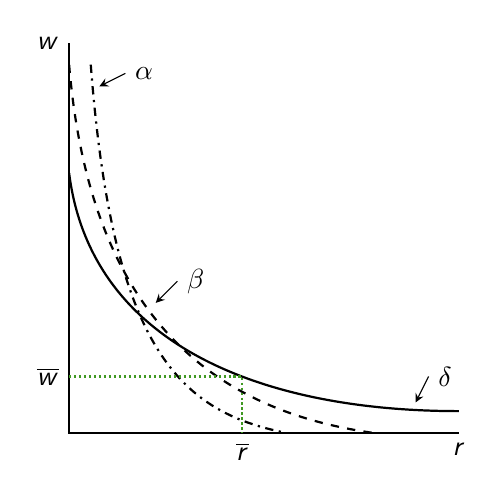
\begin{tikzpicture}[scale=0.55]
			\draw [thick] (0,9) node[left]{\(w\)} -- (0,0) -- (9,0) node[below]{\(r\)};
			\draw [thick] (0,6) .. controls (0.5,2) and (4.5,0.5) .. (9,0.5);
			\draw[<-] (8,0.7) -- (8.3,1.3) node[right]{\( \delta \)};
			\draw [thick,dashed] (0,8.5) .. controls (0.5,2.5) and (3.5,0.5) .. (7,0);
			\draw[<-] (2,3) -- (2.5,3.5) node[right]{\( \beta \)};
			\draw [thick,dash dot] (0.5,8.5) .. controls (1,2) and (2.5,0.5) .. (5,0);
			\draw[<-] (0.7,8) -- (1.3,8.3) node[right]{\( \alpha \)};
			\draw [thick, densely dotted, mygreen] (0,1.3) node [left, black] {\(\overline{w}\)}-- (4,1.3) -- (4,0) node [below, black]{\( \overline{r} \)};
		\end{tikzpicture}
	\end{figure}
	\begin{itemize}
		\item Note: adjacent techniques at a switch point will in general differ in the method of producing \myuline{only one} of the commodities
		\item \( \implies \) in the 2-commodity case, at the switch point there are three unknowns between the two price systems -- \( p_{21}, w_1 \) and \( r \)
		\item At \( r = \overline{r_1} \)
		\begin{align*}
			( a_{11}^\beta +  a_{21}^\beta p_{21} ) (1 + r) + w_1 l_1 &= 1 \\
			( a_{12}^\beta +  a_{22}^\beta p_{21} ) (1 + r) + w_1 l_2 &= p_{21} \\
			( a_{11}^\delta +  a_{21}^\delta p_{21} ) (1 + r) + w_1 l_1 &= 1 \\
			( a_{12}^\delta +  a_{22}^\delta p_{21} ) (1 + r) + w_1 l_2 &= p_{21}
		\end{align*}
		\item \( \implies \) require three equations from the two systems \( \implies \) only one equation can be different between the two systems
		\item Applying this choice of technique analysis to basic commodities, a lower price for one commodity under one method \( \implies \) a lower price for all commodities using that method
		\item \(\implies  \) ranking of techniques according to profitability as \textit{w} falls and \textit{r} rises is the same regardless of the numeraire
		\item Moreover, the ranking of techniques is independent of the technique in which prices are expressed 
		\item e.g. at \( r^* \) the relative cheapness of techniques \( \delta \) and \( \beta \) should be the same whether costs of production are compared using \( p^\delta \) or \( p^\beta \)
		\item \( \implies \) at \( r^* \) using either the real wage \( w^\beta \) or \( w^\delta \) to calculate prices for each technique would show that technique \( \delta \) yields lower prices than technique \( \beta \)
	\end{itemize}
	\begin{figure}[H]
		\centering
		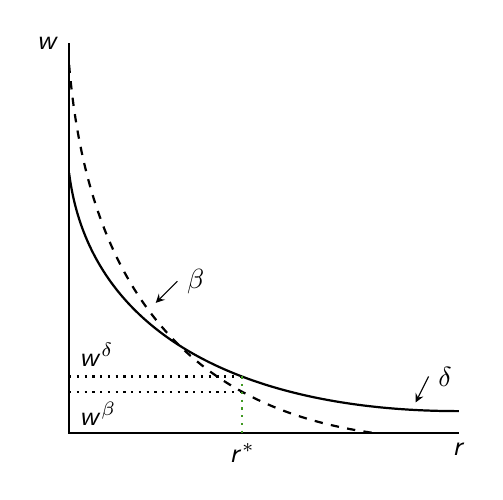
\begin{tikzpicture}[scale=0.55]
			\draw [thick] (0,9) node[left]{\(w\)} -- (0,0) -- (9,0) node[below]{\(r\)};
			\draw [thick] (0,6) .. controls (0.5,2) and (4.5,0.5) .. (9,0.5);
			\draw[<-] (8,0.7) -- (8.3,1.3) node[right]{\( \delta \)};
			\draw [thick,dashed] (0,8.5) .. controls (0.5,2.5) and (3.5,0.5) .. (7,0);
			\draw[<-] (2,3) -- (2.5,3.5) node[right]{\( \beta \)};
			\draw [thick, dotted] (0,1.3) node [above right]{\(w^\delta\)} -- (4,1.3);
			\draw [thick, dotted] (0,0.95) node [below right]{\(w^\beta\)} -- (4,0.95);
			\draw [thick, dotted, mygreen] (4,1.3) -- (4,0) node [below, black]{\( r^* \)};
		\end{tikzpicture}
	\end{figure}
	\begin{itemize}
		\item \( \implies \) at \( r^* \) using either the real wage \( w^\beta \) or \( w^\delta \) to calculate prices for each technique would show that technique \( \delta \) yields lower prices than technique \( \beta \)
		(see for example, Garegnani, 1970, p. 411n)
		\begin{figure}[H]
			\centering
			\begin{tikzpicture}[scale=0.55]
				\draw [thick] (0,9) node[left]{\(f(k)\)} -- (0,0) -- (9,0) node[below]{\(k\)};
			\end{tikzpicture}
		\end{figure}
		\item Suggests the technique which would dominate in a long-period equilibrium, for a given rate of profit, generates the highest real wage
		\item \( \implies \) \textit{dominant technique will be the technique generating the highest rate of profit at the given real wage or the highest real wage at the given rate of profit}
		\item Suggests that the relevant portion of the set of \textit{w-r} curves (representing available techniques) is the outermost envelope of this set
	\end{itemize}
	\begin{figure}[H]
		\centering
		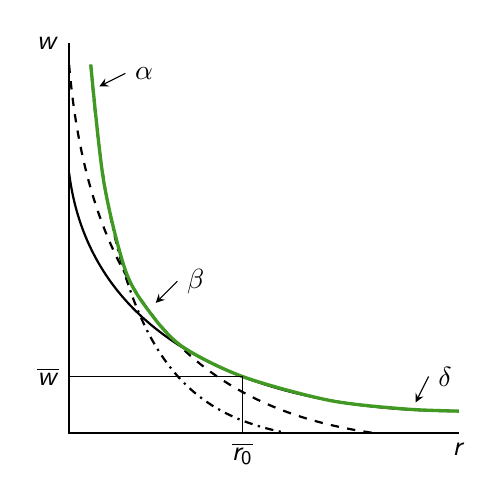
\begin{tikzpicture}[scale=0.55]
			\draw [thick] (0,9) node[left]{\(w\)} -- (0,0) -- (9,0) node[below]{\(r\)};
			\draw [thick] (0,6) .. controls (0.5,2) and (4.5,0.5) .. (9,0.5);
			\draw[<-] (8,0.7) -- (8.3,1.3) node[right]{\( \delta \)};
			\draw [thick,dashed] (0,8.5) .. controls (0.5,2.5) and (3.5,0.5) .. (7,0);
			\draw[<-] (2,3) -- (2.5,3.5) node[right]{\( \beta \)};
			\draw [thick,dash dot] (0.5,8.5) .. controls (1,2) and (2.5,0.5) .. (5,0);
			\draw[<-] (0.7,8) -- (1.3,8.3) node[right]{\( \alpha \)};
			\draw [smooth,very thick,mygreen] plot coordinates {(0.5,8.5)(0.8,5.8)(1.3,3.75)(1.85,2.8)(2.6,2)(4,1.3)(6,0.75)(7.75,0.55)(9,0.5)};
			\draw (0,1.3) node [left] {\(\overline{w}\)}-- (4,1.3) -- (4,0) node [below]{\( \overline{r_0} \)};
		\end{tikzpicture}
	\end{figure}
	\begin{itemize}
		\item Recall the discussion of duality from Section \ref{sec:1}: for every technique yielding a \( w-r \) relation there is a corresponding \( c_{w-g} \) relation
		\item \( \implies \) technological frontier of income distribution \( (w-r) \)  possibilities should correspond to the technological frontier of consumption-growth possibilities
		\item Recall also that for a given \( g = \overline{g} \) the corresponding point on the frontier indicate the technique which maximises \( c_w \) for that growth rate
	\end{itemize}
	\begin{figure}[H]
		\centering
		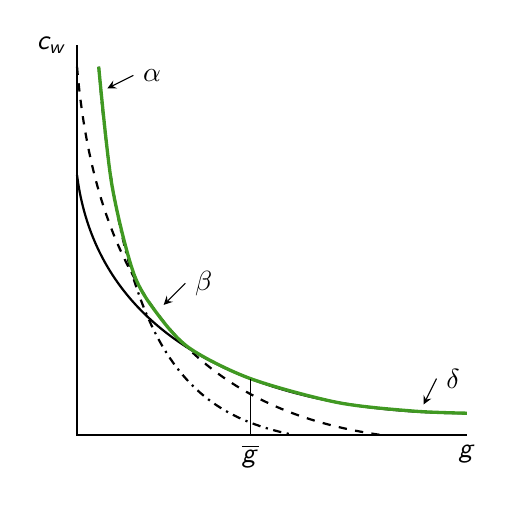
\begin{tikzpicture}[scale=0.55]
			\draw [thick] (0,9) node[left]{\(c_w\)} -- (0,0) -- (9,0) node[below]{\(g\)};
			\draw [thick] (0,6) .. controls (0.5,2) and (4.5,0.5) .. (9,0.5);
			\draw[<-] (8,0.7) -- (8.3,1.3) node[right]{\( \delta \)};
			\draw [thick,dashed] (0,8.5) .. controls (0.5,2.5) and (3.5,0.5) .. (7,0);
			\draw[<-] (2,3) -- (2.5,3.5) node[right]{\( \beta \)};
			\draw [thick,dash dot] (0.5,8.5) .. controls (1,2) and (2.5,0.5) .. (5,0);
			\draw[<-] (0.7,8) -- (1.3,8.3) node[right]{\( \alpha \)};
			\draw [smooth,very thick,mygreen] plot coordinates {(0.5,8.5)(0.8,5.8)(1.3,3.75)(1.85,2.8)(2.6,2)(4,1.3)(6,0.75)(7.75,0.55)(9,0.5)};
			\draw (4,1.3) -- (4,0) node [below]{\( \overline{g} \)};
		\end{tikzpicture}
	\end{figure}
	\begin{mybox}
		In the golden-rule case \( (r=g) \) technique which maximises \( c_w \) is also cost-minimizing
	\end{mybox}
	\begin{itemize}
		\item At the rate of profit, \( r \), under competitive conditions, technique \( \delta \) would dominate
		\item However with the growth rate given at \( \overline{g} \) the technique which maximises consumption per worker (and consumption per head) is \( \beta \)
		\item \( \implies \) ``optimal'' technique need not correspond with the cost-minimizing technique under competitive conditions
	\end{itemize}
	\begin{figure}[H]
		\centering
		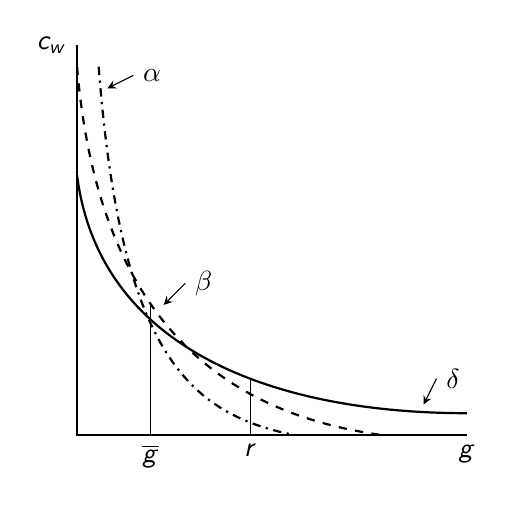
\begin{tikzpicture}[scale=0.55]
			\draw [thick] (0,9) node[left]{\(c_w\)} -- (0,0) -- (9,0) node[below]{\(g\)};
			\draw [thick] (0,6) .. controls (0.5,2) and (4.5,0.5) .. (9,0.5);
			\draw[<-] (8,0.7) -- (8.3,1.3) node[right]{\( \delta \)};
			\draw [thick,dashed] (0,8.5) .. controls (0.5,2.5) and (3.5,0.5) .. (7,0);
			\draw[<-] (2,3) -- (2.5,3.5) node[right]{\( \beta \)};
			\draw [thick,dash dot] (0.5,8.5) .. controls (1,2) and (2.5,0.5) .. (5,0);
			\draw[<-] (0.7,8) -- (1.3,8.3) node[right]{\( \alpha \)};
			\draw (4,1.3) -- (4,0) node [below]{\( r \)};
			\draw (1.7,3) -- (1.7,0) node [below]{\( \overline{g} \)};
		\end{tikzpicture}
	\end{figure}
\afterpage{\blankpage}

\section{Growth and Issues in Capital Theory}
\subsection{Distribution, Input Proportions and the Choice of Technique}
	\begin{itemize}
		\item Challenge to orthodox growth theory (Solow-Swan) in the 1950's and 1960's
		\item Based to a significant extent on criticism of orthodox capital theory \( \implies \)
		\begin{enumerate}[(i)]
			\item attack on the notion of an aggregate production function
			\item attack on orthodox view of the relation between relative factor prices and factor proportions
			\item attack on marginal productivity theory as a basis for the theory of distribution
		\end{enumerate}
		\item In general, in a competitive capitalist economy the technique in use is lowest cost
		\item Cost of production of a particular technique depends on relative prices
		\item Relative prices depend on income distribution
		\item Do techniques as well as factor proportions change in an orderly way as the distribution of income - i.e \( w \) and \( r \)-changes?
		\item Criticism between the mid-1950's and early 1970's suggests this cannot be assumed for a multi-commodity economy
		\item Significant implications for traditional (and arguably more recent) orthodox growth theory
		\item Consider a simplified corn-machine model, with only labour and a machine used as inputs
		\begin{align}
			a_c p_m (1 + \delta) + w_m l_1 &= p_c \notag \\
			a_m p_m (1 + \delta) + w_m l_2 &= p_m \label{eq:5.1}
		\end{align}
		\item With corn as numeraire and assuming everlasting machines
		\begin{align}
			a_c p_{mc} + w l_c &= 1 \notag \\
			a_m p_{mc} + w l_m &= p_{mc} \label{eq:5.2}
		\end{align}
		\item where
		\begin{equation}
			w = \frac{1 - a_m r}{l_c + r (1_m a_c - l_c a_m)} \label{eq:5.3}
		\end{equation}
		and
		\begin{equation}
			\frac{dw}{dr}  = - \frac{a_c l_m}{[l_c + r(l_m a_c - l_c a_m)]^2} < 0 \label{eq:5.4}
		\end{equation}
		and
		\begin{equation}
			p_{mc} = \frac{l_m}{l_c + r (l_m a_c - l_c a_m)} \label{eq:5.5}
		\end{equation}
		so that
		\begin{equation}
			\frac{dp_{mc}}{dr} = \frac{1_m (l_c a_m - l_m a_c)}{[l_c + r(l_m a_c - l_c a_m)]^2} \label{eq:5.6}
		\end{equation}
		\item It follows from \cref{eq:5.6} that
		\begin{equation}
			\frac{dp_{mc}}{dr} \gtreqless 0 \quad \text{where} \quad l_c a_m - l_m a_c \gtreqless 0 \label{eq:5.7}
		\end{equation}
		\item and therefore
		\begin{equation}
			\frac{dp_{mc}}{dr} \gtreqless 0 \quad \text{where} \quad \left( \frac{a_m}{l_m} \right) \gtreqless \left( \frac{a_c}{l_c} \right) \label{eq:5.8}
		\end{equation}
		\item For the quantity system, with a constant growth rate, \( g \), and writing all quantities as ratios to total labour employed in the economy
		\begin{align}
			l_m (g + \delta) M_L + l_c c &= 1 \notag \\
			a_m (g + \delta) M_L + a_c c &= M_L \label{eq:5.9}
		\end{align}
		\item where \( M_L \) is the stock of machines (per unit of labour employed in the economy) in place at the end of a period and \( (g + \delta) M_L \) is the gross investment demand for machines per unit of labour
		\item \( \implies (g+ \delta) M_L \) is output of new machines per unit of aggregate labour employment, call it \( Y_m / L \) 
		\item `\( c \)' \( \implies \) output of corn per unit of aggregate labour employment, call it \( Y_c / L \) 
		\item Decomposing \ref{eq:5.9}:
		\begin{align}
			l_m \frac{Y_m}{L} + l_c \frac{Y_c}{L} &= 1 \notag \\
			a_m \frac{Y_m}{L} + a_c \frac{Y_c}{L} &= M_L \label{eq:5.10}
		\end{align}
		\begin{align}
			\frac{L_m}{Y_m} \frac{Y_m}{L} + \frac{L_c}{Y_c} \frac{Y_c}{L} &= 1 = \frac{L_m + L_c}{L} \notag \\
			\frac{M_m}{Y_m} \frac{Y_m}{L} + \frac{M_c}{Y_c} \frac{Y_c}{L} &= M_L = \frac{M_m + M_c}{L} \label{eq:5.10}
		\end{align}
	\end{itemize}
\section{Modern Marginalist Growth Theory - ``Endogenous'' Growth Models}
\subsection{Technical progress in the Solow-Swan model}
\begin{itemize}
	\item  Simplest case: labour-augmenting (``Harrod-neutral'') technical progress. 
	\item \( \implies \) same machines, but more productive workers from one period to the next
	\item ``Effective'' labour force \( E \) grows at the rate \( g_n + \lambda \)
	\item  Production function is \( Y = (F,E) \)
	\item Relevant capital to labour ratio is now \( k_g = \frac{K}{E} \) with \( y_e = f(k_e) \) representing output per ``efficiency unit'' of labour
	\item  Steady state growth consistent with full-employment requires a constant \( k_e \) and \( y_e \)
	\item  In this situation the capital stock per worker is expanding at the same rate as labour productivity, so capital per efficiency unit of labour (i.e. \( k_e \)) is constant
	\item \( \implies \) marginal productivity of capital is constant
	\item With constant \( k_e, y_e \) is constant
	\item Maintenance of full-employment requries \( g_L = g_n \) 
	\item  But for employment to grow at this rate output must grow at a rate equal to \( g_n + \lambda \), since the quantity of labour required to produce a unit of output is falling by \( \lambda\% \) each year
	\item Hence in the steady state:
	\begin{equation}
		\frac{SY}{K} = \frac{I}{K} = g_n + \lambda \implies s \frac{\frac{Y}{E}}{\frac{K}{E}} = g_n + \lambda \implies \tcbhighmath {f(k) = \frac{(g_n + \lambda) k_e}{s}} \label{eq:6.1}
	\end{equation}
	\item \( \implies \) growth in steady state output per worker and capital per worker equal to the exogenous rate of growth of labour productivity
	\item  Exogenous technical progress can ``overcome'' diminishing returns and generate long-run growth in output per head
\end{itemize}
\begin{figure}[H]
	\centering
	\begin{tikzpicture}[scale=0.55]
		\draw [thick] (0,9) node[left]{\(f(k)\)} -- (0,0) -- (9,0) node[below]{\(k\)};
	\end{tikzpicture}
\end{figure}
\subsection{Marginalist growth theory and ``convergence''}
\begin{itemize}
	\item Solow-Swan model suggests that for the same saving propensity, population growth and technology, growth rate of poor countries exceeds that of rich countries in the transition to the steady state 
	\begin{align}
		g &= \frac{I}{K} = \frac{SY}{K} = s \frac{\frac{Y}{L}}{\frac{K}{L}} \notag \\ 
		g &= \frac{sf(k)}{k} = \frac{sy}{k} \label{eq:6.2}
	\end{align}
	\item S-S model also suggests however that poorer countries need not have a higher transition g if their `\( s \)' is lower (e.g. sP)
\end{itemize}
\begin{figure}[H]
	\centering
	\begin{tikzpicture}[scale=0.55]
		\draw [thick] (0,9) node[left]{\(f(k)\)} -- (0,0) -- (9,0) node[below]{\(k\)};
	\end{tikzpicture}
\end{figure}
\begin{itemize}
	\item  More generally, Solow-Swan model would suggest that if technology is shared, differences in steady state growth rates should reflect only differences in \( g_n \) 
	\item \( \implies \) ``conditional convergence hypothesis''
	\item Suggests also that `\( s \)' does not influence steady state growth rate of output per head 
	\item  Some have argued that evidence does not support the latter suggestion - viz., \( s \) appears to influence growth in output per head
	\item \( \implies \) development of ``endogenous'' growth model, where growth is not governed by an ``endogenous'' changes in technology
\end{itemize}
\subsection{Endogenous growth theory}
\begin{itemize}
	\item Representative agent is assumed to maximise the following intertemporal utility function
	\begin{equation}
		\int_{0}^{\infty} e^{-\rho t} u(c_t) \,\mathrm{d}t = \int_{0}^{\infty} e^{-\rho t} \frac{1}{1-\sigma}(c^{1-\sigma} - 1) \,\mathrm{d}t
	\end{equation}
	such that
	\begin{equation}
		y_t = f(k) = c_t + \Delta k_t + \delta k_t
	\end{equation}
	\item The optimum consumption plan will entail that capital per worker and consumption per worker both growth at the rate given by 
	\begin{align}
		\frac{\Delta k_t}{k_t} = \frac{\Delta c_t}{c_t} &= (\frac{1}{\sigma}f^\prime(k) -\rho - \delta) \label{eq:6.5}\\
		&\implies \rho + \left( \rho \frac{\Delta c_t}{c_t} \right) = f^\prime(k) -\delta \label{eq:6.6}
	\end{align}
	\item What is the meaning of \cref{eq:6.6}?
	\item \( \sigma \implies \) elasticity of marginal utility with respect to a given proportionate increase in per capita consumption
	\item \( \implies \sigma \frac{\Delta c_t}{c_t} \) shows the decrease in marginal utility as consumption per head grows from one period to the next
	\item \( \rho + \left( \rho \frac{\Delta c_t}{c_t} \right) \) represents the `cost' of deferring consumption from the present into the future
	\item Hence \( \rho + \left( \rho \frac{\Delta c_t}{c_t} \right) = f^\prime(k) -\delta \implies \) cost of deferring consumption is equal to the gain from additional saving
	\item  With zero population growth, the question is why there would be steady state growth in output and the capital stock?
	\item Consider the ``AK'' model: linear production function
	\begin{equation}
		Y = f(k) = AK \label{eq:6.7}
	\end{equation}
	\begin{equation}
		MP_K = f^\prime(k) = A \quad r = A -\delta \label{eq:6.8}
	\end{equation}
	\item Substituting for \( f^\prime(k) \) in equations \ref{eq:6.5} and \ref{eq:6.6} yields for the steady state growth rate
	\begin{equation}
		g = \frac{1}{\sigma} (A -\rho -\delta) \quad \therefore g = \frac{r-\rho}{\sigma} \label{eq:6.9}
	\end{equation}
	\item Given the elasticity of substitution between present and future consumption (and hence \( \sigma \)), the rate of accumulation is governed by the rate of profit compared with the discount rate
	\item The endogenous case of saving with the technology of the AK model (assuming \( \delta = 0 \))
	\begin{equation}
		s = \frac{I}{Y} = \frac{\Delta K}{K}\frac{K}{Y} = \frac{\Delta k}{k}\frac{K}{Y} = \frac{1}{\sigma}\frac{1}{A}(A -\rho)
	\end{equation}
	so that
	\begin{equation}
		g = \frac{1}{\sigma} (A - \rho) = sA = sr \label{eq:6.11}
	\end{equation}
	\item With \( s \) and \( r \) determined independently of \( g \), then both \( g \) and hence the \textbf{growth rate of output per head are ``endogenous''}
	\item With the saving ratio set exogenously
	\begin{equation}
		\frac{I}{K} = s \frac{Y}{K} = s(A) = sr \label{eq:6.12}
	\end{equation}
\end{itemize}
\subsection{Endogenous growth with human capital: Lucas}
\begin{itemize}
	\item Emphasis on positive externalities associated with the accumulation of human capital
	\item In the absence of such externalities the production function is
	\begin{equation}
		Y = AK^\beta [uhL]^{1-\beta} \label{eq:6.13}
	\end{equation}
	\item With the positive ``spin-off'' associated with accumulating human capital the production function becomes
	\begin{equation}
		Y = AK^\beta [uhL]^{1-\beta} h^{\ast\gamma} \label{eq:6.14}
	\end{equation}
	\item with the average ``quality'' of labour `\( h \)' growing according to the expression:
	\begin{equation}
		\frac{\Delta h}{h} = \upsilon(1-u) \label{eq:6.15}
	\end{equation}
	\item \( 1 - u \implies \) \% of non-lesiure time in education
	\item With the intertemporally optimising representative agent, steady state growth in output per worker is given by (Sala-i-Martin, 1990) 
	\begin{equation}
		g = \frac{(\upsilon - \rho)(1-\beta)}{\sigma(1+\gamma-\beta)} = \frac{\Delta c}{c} = \frac{\Delta k}{k} \label{eq:6.16}
	\end{equation}
	\item Note, in the absence of the externatlity (i.e. \( \gamma = 0 \)) \cref{eq:6.16} simplifies to
	\begin{equation}
		g = \frac{\upsilon - \rho}{\sigma} \label{eq:6.17}
	\end{equation}
	\item Note the similarity with \cref{eq:6.9} for the AK model
	\item The steady state growth rate of human capital depends on the nature of the externality, specifically, on the coefficient \( \gamma \) so that
	\begin{equation}
		\frac{\Delta h}{h} = \frac{\Delta k}{k} \frac{(1-\beta)}{(1 + \gamma - \beta)} \label{eq:6.18}
	\end{equation}
	\item If \( \gamma = 0 \), \( \frac{\Delta h}{h} = \frac{\Delta k}{k} \)  
	\item Endogenous growth models however retain a couple of troublesome features of earlier marginalist growth theory:
	\begin{itemize}
		\item failure to consider effective demand, reflected in the assumed relation between \( S \) and \( I \);
		\item the use of aggregate production functions to represent multi-commodity systems
	\end{itemize}
\end{itemize}
\section{``Cambridge'' growth theory and modern post-Keynesian / Kaleckian Models}
\subsection{Cambridge growth theory}
	\begin{itemize}
		\item Early Cambridge/post-Keynesian analysis (1950's -- 60's):
		\begin{itemize}
			\item heavily influenced by Keynes and Kalecki: accept a demand-driven view of output
			\item rejection of marginal productivity theory of distribution
			\item dissatisfaction with the uniqueness of Harrod's warranted growth path (though not the notion that \( g_w \) need not to coincide with \( g^n \))
		\end{itemize}
	   \item Along the warranted path producers accumulate capital at the rate \( \frac{s}{v} \)
	   \item If their actual rate differs from \( \frac{s}{v} \implies \) instability in Harrod's analysis
	   \item For early Cambridge theorists 
	   \begin{itemize}
		\item `\( s \)' depended on distribution between wages and profits; 
		\item distribution was influenced by the rate of growth, in particular `\( r \)' was influenced by `\( g \)'
	   \end{itemize}
	   \item Hence if \( \frac{I}{K} > \frac{s}{v} \) the higher growth rate could become the warranted path if `\( r \)' increased and in turn `\( s \)'
	   \item \( \implies g_w \) is no longer unique
	   \item  Cambridge theorists arrived at the so-called Cambridge equation
	   \begin{equation}
			g = s_c r \label{eq:7.1}
	   \end{equation}
	   \item \textit{Causation is seen to run from left to right -- `\( g \)' is exogenous and determines `\( r \)'} 
	\end{itemize}
\subsection{Modern Post-Keynesian/Kaleckian Models}
	\begin{itemize}
		\item Modern Kaleckian theorists take `\( g \)' as endogenous, by combining the Cambridge growth \cref{eq:7.1} with an explanation of the rate of accumulation
		\item Consider a stylised one-sector version of modern post-Keynesian/Kaleckian ``growth'' models
		\begin{equation}
			p = wl\varphi \quad\text{with}\quad \varphi>1 \label{eq:7.2}
		\end{equation}
		\item Profit share \( \pi \) is given by
		\begin{equation}
			\pi = \frac{p-wl}{p} = 1-\frac{w}{p}l = \frac{\varphi-1}{\varphi} \label{eq:7.3}
		\end{equation}
		\item Profit rate \( r \) is given by
		\begin{equation}
			r=\left(\frac{p-wl}{p}\right)\frac{Y}{K} = \left( \frac{\varphi-1}{\varphi} \right) u = \pi u \label{eq:7.4}
		\end{equation}
		\item The rate of accumulation which would absorb exactly the flow of savings is
		\begin{equation}
			g^s - s_c r \left( =\frac{S}{\pi}\frac{\Pi}{K} \right) \label{eq:7.5}
		\end{equation}
		\item On the basis of an investment function like
		\begin{equation}
			I_t = A + \alpha\Pi_t + \beta Y_t - \gamma K_t \label{eq:7.6}
		\end{equation}
		\item one can write (dividing throigh by K) a ``desired accumulation'' function in the form
		\begin{equation}
			g^i = f_0 + f_1r + f_2u_t \label{eq:7.7}
		\end{equation}
		\item For equilbrium growth \( g^s = g^i \)
		\begin{equation}
			\implies \frac{S}{K}=\frac{I}{K} \quad\text{and therefore}\quad s_c r = f_0+f_1r+f_2 u_t \label{eq:7.8}
		\end{equation}
		\item Substituting \( \pi u \) for \( r \) in \cref{eq:7.7} gives
		\begin{equation}
			s_c\pi u = f_0 + f_1 \pi u + f_2 u \label{eq:7.9}
		\end{equation}
		\item and therefore steady-state \( u \) is given by
		\begin{equation}
			u^*=\frac{f_0}{(s_c - f_1)\pi - f_2} \label{eq:7.10}
		\end{equation}
		\item Stability of steady state growth requires saving to react to changes in utilisation more than investment
		\item \( \uparrow s_c \) leads to a fall in \( g^*, u^* \) and \( r^* \implies \) ``paradox of thrift''
	\end{itemize}
	\begin{figure}[H]
		\centering
		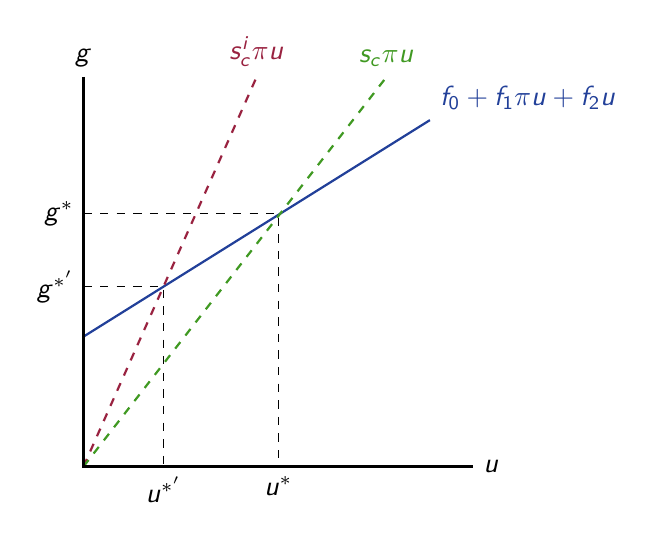
\begin{tikzpicture}[scale=0.55]
			\draw [thick,color=myblue] (0,3) -- (8,8) node [above right] {\( f_0+f_1\pi u + f_2 u \)};
			\draw [thick,dashed,color=myred] (0,0) -- (4,9) node [above] {\( s_c^i\pi u \)};
			\draw [thick,dashed, color=mygreen] (0,0) -- (7,9) node [above] {\( s_c\pi u \)};
			\draw [dashed] (0,4.15) node [left] {\( g^{*^\prime} \)} -- (1.85,4.15) -- (1.85,0) node [below] {\( u^{*^\prime} \)};
			\draw [dashed] (0,5.85) node [left] {\( g^{*} \)} -- (4.5,5.85) -- (4.5,0) node [below] {\( u^{*} \)};
			\draw [thick] (0,9) node [above]{\( g \)} -- (0,0) -- (9,0) node [right]{\( u \)};
		\end{tikzpicture}
	\end{figure}
	\begin{itemize}
		\item In this model a (assuming a stable \( g^* \)) shift in distribution towards profit reduces utilisation, the profit rate and \( g^* \) - referred to as the ``stagnationist'' case
		\item This case has non-orthodox implications about the relation between the real wage and employment. From \cref{eq:7.10}
		\begin{equation}
			\frac{\mathrm{d} u^*}{\mathrm{d} \pi} = \frac{-(s_c-f_1)f_0}{[(s_c-f_1)\pi-f_2]^2} \label{eq:7.11}
		\end{equation}
		\item Since, for stability, \( f_1,\pi + f_2 \leq s_c\pi \), and thus \( \frac{f_2}{\pi} < (s_c-f_1) \), then, with \( f_2 \) and \( \pi > 0 \), \( (s_c-f_1) > 0 \) and thus \( \frac{\mathrm{d} u^*}{\mathrm{d} \pi} < 0 \)
		\item In turn, since
		\begin{equation}
			I = \frac{L}{Y}\frac{Y}{K}K=l\cdot u \cdot K \label{eq:7.12}
		\end{equation}
		\item \( \implies L \)  per unit of \( K \) rises with utilisation, and thus with a fall in \( \pi \) and thus with a \textbf{rise} in the real wage \( \frac{w}{P} \)
		\item This case also suggests a positive relation between the steady state rate of profit and the real wage 
		\item i.e. a fall in the profit share -- rise in the real wage -- increases aggregate demand, utilisation and accumulation
		\item The increase in utilisation outweighs effect of a fall in \( \pi \) on the rate of profit, \( r \),  so that \( r \) rises
		\item Hence rate of return to capital and growth are stimulated by a shift in distribution towards wages
		\item Argument by later theorists in the post-Keynesian Kaleckian tradition that the model above exaggerated the effects of changes in utilization rates \( (u) \) on investment demand
		\item A more general alternative suggested for the desired accumulation function was
		\begin{equation}
			g^i = h(\pi,u) \quad h_{\pi},h_u>0 \label{eq:7.13}
		\end{equation}
		\item \( \implies \) an increase in profit share, for a given utilisation and an increase in utilisation for a given profit share would both increase the desired rate of accumulation
		\item  Steady state utilisation rate is the solution to
		\begin{equation}
			s_c\pi u = h(\pi,u) \quad\text{with}\quad \frac{du}{d\pi} = \frac{-\left( s_cu-h_{\pi} \right)}{s_c\pi-h_u} \label{eq:4.33}
		\end{equation}
		\item Stability of the steady state requires
		\[
			s_c\pi-h_u>0
		\]
		\item Whether `\( u^* \)' rises or falls with a rise in the profit share turns on whether \( s_c u-h_{\pi} \) is < 0 or > 0
		\item If \( s_c u-h_{\pi} > 0, \frac{du}{d\pi}<0 \implies \) ``stagnationist'' case
		\item Although a rise in the profit share, \( \pi \), has a positive effect, \textit{ceteris paribus}, on the desired rate of accumulation (and potentially on \( u \)), there is a greater negative effect on utilisation (via the fall in the real wage depressing consumption demand)
		\item \( \implies \) negative impact on the steady state rate of accumulation and on the steady state rate of profit
		\item Alternative possibility, referred to in the literature as the ``exhilarationist'' case
		\item Suppose that \( s_c\pi-h_u<0 \), then \( \frac{du}{d\pi}>0 \)
		\item \( \implies \) a redistribution of income towards profits has a net stimulatory effect on aggregate demand
		\item \( \implies \) stimulus to utilisation via the positive effect of a rise in \( \pi \) on capitalists' consumption and accumulation outweighs negative impact on utilisation from a falling real wage reducing workers' consumption
		\item The steady state rate of accumulation and the steady state rate of profit both rise
		\item These different cases entail two different relations between steady state distribution and the steady state
		\item The stagnationist case: a rise in \( g^* \), a fall in the \( \pi \) and \myuline{a rise in the real wage}, steady state utilisation \myuline{and rate of profit}
		\item The exhilarationist case: a rise in \( g^* \), a rise in \( \pi \), \myuline{a fall in the real wage, a rise in the rate of profit} and a rise in steady state utilisation
		\item The ``stagnationist'' case may also be referred to as ``wage-led'' growth while the ``exhilarationist'' case may be referred to as ``profit-led'' growth
		\item As Blecker (2003) notes, there are intermediate cases between the stagnationist and exhilarationist possibilities 
	\end{itemize}
\section{Growth and Policy}
\subsection{Concluding Remarks}
\begin{itemize}
	\item What, if any, policy implications can be drawn from the discussion in previous sections.
	\item Have noted two ``grand traditions'' in growth theory
	\item Generate different perspectives on policy
	\item In relation to marginalist growth theory (Solow-Swan, endogenous growth models (EGT)) - ??
	\item In Solow-Swan: assuming a higher growth rate is desirable \( \implies \) increasing the growth rate of the labour force and/or rate of technical progress
	\item Both are exogenous; though policy makers could make use of labour market policies which increase gn and policies to stimulate productivity?
	\item Note: higher long-run growth rate is not to prevent rising unemployment -- this is not a long-run problem with flexible factor prices and competitive factor markets
	\item \( \implies \) possible role for micro-based policy?
	\item Higher steady state growth may be desired for long-run increases in income per capita
	\item If the object is to maximise consumption per head \( \implies \) a role for saving in the Solow-Swan model
	\item \( \implies \) a role for policy designed to influence saving (e.g. pensions, superannuation) depending on initial situation (i.e. economy is initially dynamically efficient or inefficient)
	\item However in EGT, in contrast to Solow-Swan, saving has a role in governing the long-run growth rate
	\item EGT suggests also a role for policy in enhancing growth in human capital (education policy)
	\item Also potentially a role for industry/innovation policy?
	\item So what of non-orthodox growth theory -- Harrod-Domar, post-Keynesian/Kaleckian models?
	\item More immediate implication of modern post-Keynesian/Kaleckian models of a role for distribution
	\item But how? Effect on steady state growth of shifting distribution between wages and profits turns on parameters 
	\item i.e. depends whether growth is wage or profit-led
	\item More generally with both old and new non-orthodox models -- growth is demand-driven!
	\item And there is no presumption of a mechanism bringing \( g^\ast \)  into line with \( g^n \) 
	\item \( \implies \) a role for policy in adjusting growth to deal with unemployment
	\item \textbf{AND} (in light of the capital-theoretic criticisms of orthodox theory) regardless of the competitiveness of factor markets, esp. the labour market
	\item \( \implies \) a role potentially for policy in manipulating the rate of growth of aggregate demand
	\item \( \implies \) completely contrasting to marginalist growth theory which would not see demand as a constraint on long-run growth
\end{itemize}
\subsection{Demand-Led Theory of Growth -- the ``supermultiplier approach''}
\begin{itemize}
	\item A relatively recent view of growth as a demand-led process is the so-called ``supermultiplier'' approach
	\item Consists of extending the Keynesian short-run theory of output to a long-run theory of output growth. In the long run the growth of productive capacity adjusts to the requirements of demand growth
	\item In this theory the growth of output, employment and capital depend on the growth in aggregate demand where the growth path is not characterised by the full-employment of labour 
	\item Capacity adjustment is incorporated by way of the accelerator theory of investment
	\item From the basic Keynesian income-expenditure model
	\begin{equation}
		AE = A + (c - ct - m) Y + I \label{eq:8.1}
	\end{equation}
	\item Induced investment is given by:
	\begin{equation}
		I_t = v (Y_{t+1}^e - Y_t) \label{eq:8.2}
	\end{equation}
	\item In turn
	\begin{equation}
		AE = A + (c - ct - m) Y + \nu (Y_{t+1}^e - Y_t) \label{eq:8.3}
	\end{equation}
	In equilibrium, \( Y = AE \) so that
	\begin{equation}
		Y_t = A_t + c^d Y_t + \nu (Y_{t+1}^e - Y_t) \label{eq:8.4}
	\end{equation}
	where \( c^d = (c - ct - m) \) is the propensity to spend on domestically produced goods.
	\item The expected growth rate is given by
	\begin{equation}
		g_{t+1}^e = \frac{\left( Y_{t+1}^e - Y_t \right)}{Y_t} \label{eq:8.5}
	\end{equation}
	so that \cref{eq:8.4} can be rewritten as
	\begin{equation}
		Y_t = A_t + c^d Y_t + \nu g_{t+1}^e Y_t \label{eq:8.6}
	\end{equation}
	\item In turn
	\begin{equation}
		Y_t = A_t \frac{1}{1 - c^d - \nu g_{t+1}^e} \label{eq:8.7}
	\end{equation}
	\item \( \frac{1}{1 - c^d - \nu g_{t+1}^e} \) represents the ``supermultiplier''
	\item i.e. the multiplier effect of a change in autonomous demand `\( A \)'is not just induced consumption deman (via `\( c^d \)') but also induced investment demand (via `\( v g^e \)')
	\item Equation (8.7) implies that with a given supermultiplier, the rate of growth of output over time reflects the rate of growth of autonomous demand
	\item This approach is in the spirit of Keynes and later post-Keynesian and Kaleckian approaches in suggesting that there is no mechanism to guarantee that the growth of autonomous demand will be sufficient for the maintenance of full-employment
	\item Apart from consumption proprensities and technology (i.e. `\( \nu \)') the supermultiplier itself depends on expectations about the future rate of growth
	\item \( \implies \) implications of the supermultiplier approach depend in part on the theoretical approach regarding the formation of expectations
	\item BUT, the demand-led growth thesis raises an additional  complex theoretical question (not entirely without practical policy interest): what is the autonomous element(s) of demand which drives growth?
	\item If output and output capacity are ultimately dictated by demand, there must be an independent or autonomous component?
	\item i.e. independent of current and anticipated growth rate of income
	\item Not easy to conceive of expenditures autonomous in this sense for \myuline{all time}
	\item Problems with the concept of autonomous investment and to a lesser extent with consumption
	\item Government expenditure also less of a problem, but arguably subject to at least a long-run intertemporal government budget constraint
	\item And seen as having a one-way relation with public debt and running a sustainable fiscal policy
	\item But a demand-led approach suggests this is an over-simplified view
	\item Consider a simplified version of the standard fiscal sustainability condition:
	\[
		\frac{S}{PY} \geq - g \frac{B}{PY} \qquad \frac{S^p}{PY} \geq (i - g) \frac{B}{PY}
	\]
	\item Latter condition shows how big the primary surplus as a \% of GDP must be to prevent debt rising faster than nominal GDP
	\item \( \implies \) if \( i > g, \implies \) fiscal sustainability requires a primary budget surplus
	\item From an orthodox standpoint -- specifically, Solow-Swan -- `\( g \)' is exogenous
	\item If `\( i \)' is governed by the rate of profit then in a Solow-Swan world, `\( i \)' is governed by `\( s \)', `\( f(k) \)' and `\( g \)' 
\end{itemize}
\begin{figure}[H]
	\centering
	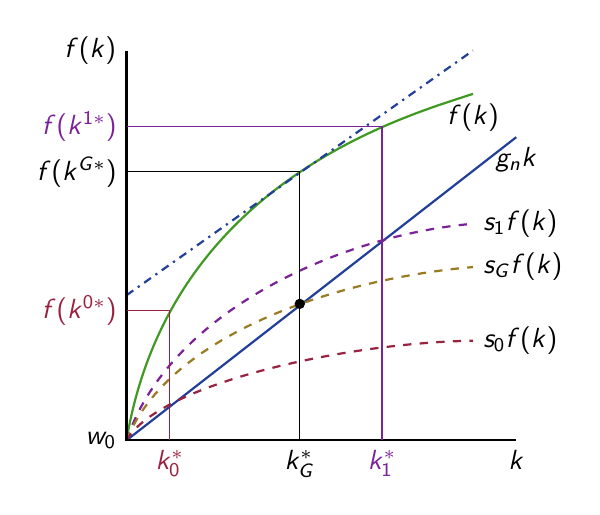
\begin{tikzpicture}[scale=0.55]
		\draw [thick, myblue] (0,0) node[left, black]{\( w_0 \)} -- (9,7) node[below, black]{\( g_n k \)};
		\draw [thick, mygreen] (0,0) .. controls (1,6) and (6.5,7.5) .. (8,8) node[below, black]{\( f(k) \)};
		\draw [thick, mypurple, dashed] (0,0) .. controls (1,3) and (5,4.75) .. (8,5) node[right, black]{\( s_1f(k) \)};
		\draw [thick, mygold, dashed] (0,0) .. controls (1,2.5) and (5,3.75) .. (8,4) node[right, black]{\( s_Gf(k) \)};
		\draw [thick, myred, dashed] (0,0) .. controls (0.75,1.3) and (5,2.25) .. (8,2.3) node[right, black]{\( s_0f(k) \)};
		\draw [thick, dash dot, myblue] (0,3.35) -- (8,9);
		\draw [thick] (0,9) node[left]{\(f(k)\)} -- (0,0) -- (9,0) node[below]{\(k\)};
		\draw [myred] (1,0) node[below]{\( k_0^{\ast} \)} -- (1,3) -- (0,3) node[left]{\( f(k^{0\ast}) \)};
		\draw [mypurple] (5.9,0) node[below]{\( k_1^{\ast} \)} -- (5.9,7.25) -- (0,7.25) node[left]{\( f(k^{1\ast}) \)};
		\draw (4,0) node[below]{\( k_G^{\ast} \)} -- (4,6.2)  -- (0,6.2) node[left]{\( f(k^{G\ast}) \)};
		\filldraw[black] (4,3.15) circle (3pt);
	\end{tikzpicture}
\end{figure}
\begin{itemize}
	\item \( \implies \) if `\( s \)' is manipulated to keep the economy in the region of ``dynamic efficiency'' so that \( (i \geq g) \) primary surplus will be required for fiscal sustainability (defined as a stable debt to income ratio)
	\item From a non-orthodox, demand-led perspective things are more complex
	\item `\( g \)' is not independent of the growth rate of govt. expenditure
	\item \( \implies \) although the primary deficit is ceteris paribus positively influenced by the govt. expenditures, so is the growth rate of nominal GDP
	\item \( \implies \) a rise in the rate of growth of govt. expenditure will ceteris paribus act negatively on `\( s^P \)' but also positively on `\( g \)' relative to `\( i \)' (assuming the economy is not too close to full-employment)
	\item Moreover, non-orthodox theorists would reject the implication of the Solow-Swan model that a change in `\( s \)' would influence `\( i \)' while either boosting `\( g \)' or leaving it unchanged
	\item \( \implies \) from non-orthodox, demand-led perspective, `\( i \)' is not governed by demand and supply of saving; but a rise in saving could depress the rate of growth of effective demand and in turn the rate of growth of output
\end{itemize}
\end{document}
